\documentclass[11pt, a4paper]{article}

\usepackage{graphicx}
\usepackage{listings}
\usepackage{color}
\usepackage{amsmath}
\usepackage{geometry}
\usepackage{setspace}
\usepackage{biblatex}
\usepackage{subfig}
\usepackage{float}

\usepackage[export]{adjustbox}
 
% Page master configuration
\lstset { basicstyle=\ttfamily, breaklines = true, tabsize=2 }
\geometry { a4paper, total={170mm,257mm}, left=20mm, top=20mm, right=20mm, bottom=20mm }
\graphicspath{{Images/}}
\addbibresource{biblography.bib}
\setlength{\parskip}{0.5em}
\setlength{\parindent}{0cm}

\definecolor{dkgreen}{rgb}{0,0.6,0}
\definecolor{gray}{rgb}{0.5,0.5,0.5}
\definecolor{mauve}{rgb}{0.58,0,0.82}

\lstset{frame=tb,
  language=Java,
  aboveskip=3mm,
  belowskip=3mm,
  showstringspaces=false,
  columns=flexible,
  basicstyle={\footnotesize\ttfamily},
  numbers=none,
  numberstyle=\tiny\color{gray},
  keywordstyle=\color{blue},
  commentstyle=\color{dkgreen},
  stringstyle=\color{mauve},
  breaklines=true,
  breakatwhitespace=true,
  tabsize=3
}

%%%%%%%%%%%%%%%%%%%%%%%%%%%%%%%%%%%%%%%%%%%%%%%%%%%%%%%%%%%%%%%%%%%%%%%%%%%%%%%%%%%%%%%%%%%%%%%%%%%%%%%%%%
\begin{document}

\begin{titlepage}
	\newcommand{\HRule}{\rule{\linewidth}{0.5mm}}
    
\includegraphics[scale=0.1]{./Images/Imperial_Logo.jpg} 
    \\
    \center 
	\textsc{\large Department of Electrical and Electronic Engineering }\\[0.5cm] 
	\textsc{\normalsize ELEC50008: Engineering Design Project}\\[0.5cm] 
    
	\HRule \\[0.4cm]
	Group 18: Mars Rover Project Report
    \HRule \\[1.5cm]
     
    \begin{center}
		\underline{Authors}\\[0.5cm] 
        Aixin Zhang \\ CID: 01738988 \\ az419@ic.ac.uk \\ [0.5cm]

        Ebby Samson \\ CID: 01737449 \\ es1219@ic.ac.uk \\ [0.5cm]
        
        Igor Dmytrovich Silin \\ CID: 01756268 \\ ids19@ic.ac.uk \\ [0.5cm]

        Kaling Ng \\ CID: 01737644 \\ kln19@ic.ac.uk \\ [0.5cm]

        Nur Izzah Mohd Zafer \\ CID: 01738670 \\ nim19@ic.ac.uk \\ [0.5cm]    
        
        Xin Wang \\ CID: 01735253 \\ xw2519@ic.ac.uk \\ [0.5cm]

	\end{center} \large

    \vfill 
    \makeatletter
    \@date 
    \makeatother
\end{titlepage}

%%%%%%%%%%%%%%%%%%%%%%%%%%%%%%%%%%%%%%%%%%%%%%%%%%%%%%%%%%%%%%%%%%%%%%%%%%%%%%%%%%%%%%%%%%%%%%%%%%%%%%%%%%
\renewcommand{\baselinestretch}{0.75}\normalsize
\tableofcontents
\renewcommand{\baselinestretch}{1.0}\normalsize

\pagebreak
%%%%%%%%%%%%%%%%%%%%%%%%%%%%%%%%%%%%%%%%%%%%%%%%%%%%%%%%%%%%%%%%%%%%%%%%%%%%%%%%%%%%%%%%%%%%%%%%%%%%%%%%%%

%%%%%%%%%%%%%%%%%%%%%%%%%%%%%%%%%%%%%%%%%%%%%%%%%%%%%%%%%%%%%%%%%%%%%%%%%%%%%%%%%%%%%%%%%%%%%%%%%%%%%%%%%%
\section{Project Management}

The project team utilised the Project Management Institute's 5 Phases of Project Management \footnote{PMI: https://www.smartsheet.com/blog/demystifying-5-phases-project-management} as a guide to ensure all aspects of project planning and management are captured in the team's project management approach. 

Project management was split into 3 areas, each covering a important section of project management.

\subsection{Conception and Initiation}

\textbf{Project definition}: Design and build a rover system that has autonomous capabilities to detect, avoid and transmit the locations of the obstacles i.e. coloured balls to a server that users can interact with.

\textbf{Project requirement}: The rover system is split into 5 modules, each with its own requirements:

\begin{itemize}
    \item Command:
    \begin{itemize}
        \item Enable bilateral communication between user and Control module 
        \item Enable users to nagivate the rover 
        \item Plot a map of the locations of the obstacles encountered by the rover   
    \end{itemize}

    \item Control:
    \begin{itemize}
        \item Enable bilateral communication channels between Command, Drive, Energy and Vision modules
    \end{itemize}
    
    \item Drive:
    \begin{itemize}
        \item Defines the operation of the two rover motors such as:
        \begin{itemize}
            \item Speed control 
            \item Direction control 
            \item Turning method 
        \end{itemize}
        \item Using the optical flow sensor, measure the distance travelled by the rover 
    \end{itemize}
    
    \item Energy:
    \begin{itemize}
        \item Battery charge operation: Profile design, status estimation and melt/explosion prevention 
        \item Battery voltage balancing and range estimation 
        \item Implementing PV MMPT calculation algorithm 
        \item Integrating and testing solar charging system  
    \end{itemize}
    
    \item Vision:
    \begin{itemize}
        \item Using the on-board camera detect, avoid and record the location of obstacles encoutered by the rover  
    \end{itemize} 
\end{itemize}


\vfill

\pagebreak
\subsection{Definition and Planning}

The project team had a significant amount of freedom in designing and developing the rover system to meet the project requirements. The team had identified several design themes that guided the design and implementation choices made during the developement of the rover system:

\begin{itemize}    
    \item \textbf{Modularity}:
    
    Having taken into account that the project team spanned four countries with different time-zones and the time constraint of the project, the team felt it was important to incorporate modular design in the development of each rover modules. 
    
    The approach meant each subsystem only had to ensure the pre-agreed connection interfaces such as WebSocket was compatible with the required modules. This was very advantageous due to the following:
    \begin{itemize}
        \item Each module could independently develop sections of the rover system. This made the team much more dynamic and efficient.
        \item The testing strategy \footnote{Testing was managed by the Integration module} was more methodical and could occur early in stages, gradually leading up to a full rover system test.
        \item No unnecessary meetings. By reducing the number of meetings the team had, it meant less time was wasted on arranging a time suitable for three time-zones and team meetings were more productive.  
    \end{itemize}

    \item \textbf{Scalability}:
    
    During the first meeting, the team was not certain as to the exact features that are desirable in a rover system. Due to this reason, scalability was a critical consideration factor and gave the team a very flexible approach to the rover system. 
    
    An example would be the MongoDB database implemented by Command. MongoDB is a type of "NoSQL" database that is not as restrictive as traditional SQL databases which allowed the team to store new types of data without having to redesign the database model. 

    \item \textbf{Open-source}: 
    
    Where possible, the team opted to use well-supported open-source development packages such as the FastAPI framework. This complimented modularity and scalability themes by ensuring the interfaces are industry-standard and could be easily modified to expand its capabilites. 
    
    Being well-supported, there is ample documentation to support the development and the codebase is well-designed. This meant that the team could reduce the number of unknown bugs, decrease development time and ensure a high-quality codebase.     

    \item \textbf{Minimalism}:
    
    Due to the open-ended nature of the project, the team did not want to limit the scope of their design but, at the same time, did not want to risk a bloated and inefficient rover system due to feature creep and badly integrated modules. 
    
    The team determined any design choice would need to prioritise efficiency and scalablity. All libraries are to be lightweight and only need to support the required features. 
    
\end{itemize}

\vfill

\pagebreak
\subsection{Performance and Control}

\subsubsection{Team communication}

\begin{figure} [h!]
    \centering
    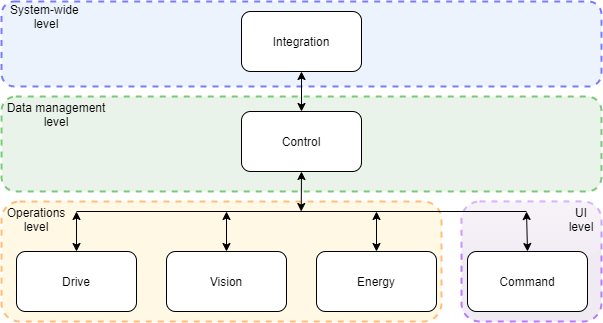
\includegraphics[scale=0.4]{Comms.png}
    \caption{Project Communication Hierarchy}
\end{figure}

During the first week of the project, the team implemented a communication hierarchy that showed the communication flow between each module and any related components between the modules. The hierarchy was split into four classifications that reflected the primary responsibility of its member modules in order to help with easily identifying the responsibilities a module had. 

The project team met twice each week on Wednesday and Sunday to ensure each module's progress was on track and the Control module was aware of any changes. The Control module was responsible for leading each session and taking the meeting minutes \footnote{Example meeting minute avaiable in appendix}. 
 

\subsubsection{Project timeline}

\begin{figure} [h!]
    \centering
    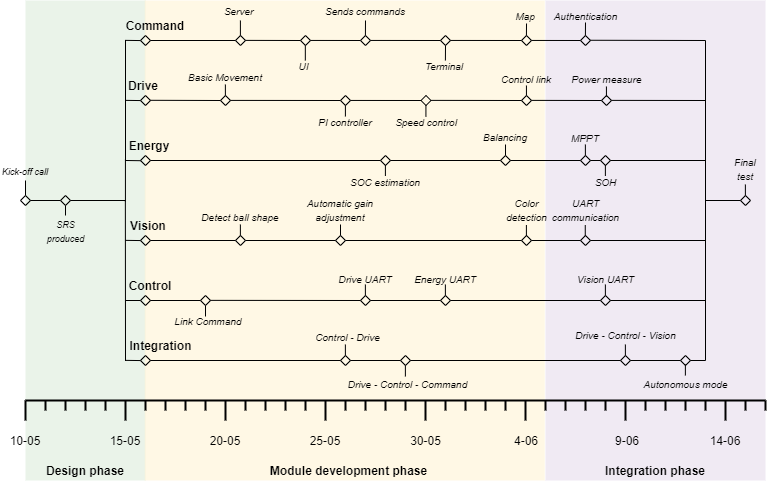
\includegraphics[scale=0.4]{Timeline.png}
    \caption{Group 18 Project Timelines}
\end{figure}

The project timeline is divided into three phases which placed priority in different aspects of the project. The Design phase included project and individual module research where the design themes are implemented. The Module developement phase was where the Integration module worked with the individual modules to test certain aspects of the module. The Integration phase was where modules are linked and tested together, gradually increasing the complexity.

With the advantage of the Gantt chart, the Integration module was able to identify which module was near testing capable and arrange with the related modules e.g. Command - Control - Drive for testing. 

\vfill
\pagebreak

\subsubsection{Gantt chart}

The project team used the Gantt chart provided at the start of the project and consistently updated it throughout the timeline of the project. With the team meeting twice a week to give updates on each module's progress, the Gantt was updated after every meeting to reflect any change in development time and any additional work. 

Due to certain complications like Quartus, the timelines of Vision and Control had to be modified several times. With the whole team having access to the Gantt chart, it allowed the team identify a module's completed feature and to more easily arrange any inter-module testing such as Command to Control to Drive.  

The team found using the Gantt chart has its advantages and disadvantages. The chart was a great place for team members to see the progress of other team members and plan their own module to coincide with certain testing milestone. On the other hand, it got quite complicated and changes occured often so team members had to constantly check the chart to see if they are in sync with modules like Control. This was mitigated by editing the Gantt chart live during each meeting so members know exactly what changed and what they need to be aware of.




\vfill
%%%%%%%%%%%%%%%%%%%%%%%%%%%%%%%%%%%%%%%%%%%%%%%%%%%%%%%%%%%%%%%%%%%%%%%%%%%%%%%%%%%%%%%%%%%%%%%%%%%%%%%%%%






%%%%%%%%%%%%%%%%%%%%%%%%%%%%%%%%%%%%%%%%%%%%%%%%%%%%%%%%%%%%%%%%%%%%%%%%%%%%%%%%%%%%%%%%%%%%%%%%%%%%%%%%%%
\pagebreak
\section{Rover system design}

\subsection{Structural design}

\begin{figure} [h!]
    \centering
    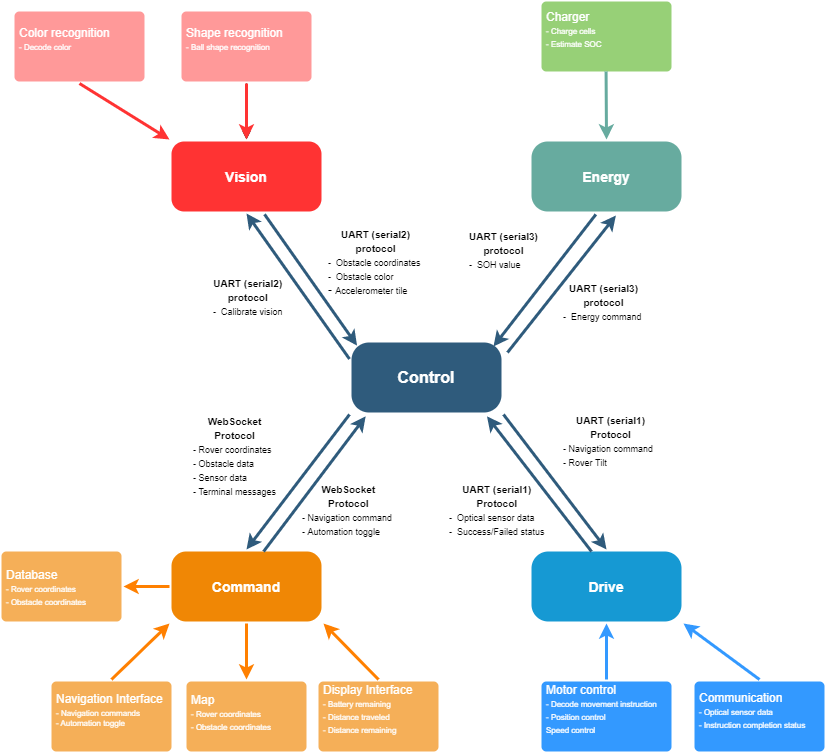
\includegraphics[scale=0.5]{Structure.png}
    \caption{Rover structural diagram}
\end{figure}

The team established the structural design of the rover system during the first week of the project timeline. The structural design is formed in three stages: 

\begin{enumerate}

    \item \textbf{Identifying the core module}: 
    
    The Control module was designated as the core module of the rover system due the ESP32 board's numerous communication interfaces and on-board data processing capabilities. With the remote nature of the project, this also meant the Control module will take the leadership role and act as the "heartbeat" of the team - ensuring each module development was in sync with the planned project timeline and each communication interface was compatible with Control.   

    \item \textbf{Module connection}:
    
    With the role of Control established, the team could discuss how to structure the other modules that best took advantage of the ESP32's capabilities, ensured efficient operation in various environments and complimented the \textit{scalability} design theme. 

    A major design problem was the location of processing the data from sensors like the optical sensor. The team chose to do as much processing locally on the ESP32 because the connection with Command module servers naturally has a certain degree of latency and Control was best equipped module on the rover to handle the processing. The Control module can also pre-process data to minimise the amount sent to Command and reduce the end-to-end latency of the system.
    
    \item \textbf{Communication interface selection}: 
    
    In the second stage, the Control module worked with each module to research and select the most suitable communication interface. This was critical to establish the interfaces early on to allow the modules to start development as soon as possible and asynchronously as mentioned with \textit{modularity} design theme. 

    The biggest concern was the type of connection between the Control module and Command server. The form of connection had to be energy efficient to compliment the \textit{minimalism} design theme and be able to scale easily depending on the data generated from the rover. The final design choice was to use the WebSocket protocol since it was native to the FastAPI framework used by Command and allowed real-time updates to the user. Compared to the HTTP protocol, the WebSocket protocol has a higher performance rating at 83 ms on WebSocket and 107 ms on HTTP for an average single request \cite{SocketvsHTTP}.  

\end{enumerate}  

\subsection{Functional design} 

\begin{figure} [h!]
    \centering
    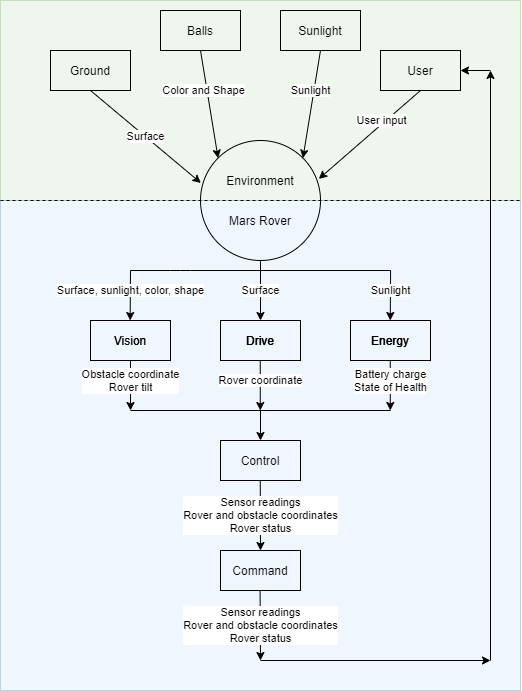
\includegraphics[scale=0.6]{Rover functional.png}
    \caption{Rover system context diagram}
\end{figure}


%%%%%%%%%%%%%%%%%%%%%%%%%%%%%%%%%%%%%%%%%%%%%%%%%%%%%%%%%%%%%%%%%%%%%%%%%%%%%%%%%%%%%%%%%%%%%%%%%%%%%%%%%%
\pagebreak
\subsection{Intellectual property}
%%%%%%%%%%%%%%%%%%%%%%%%%%%%%%%%%%%%%%%%%%%%%%%%%%%%%%%%%%%%%%%%%%%%%%%%%%%%%%%%%%%%%%%%%%%%%%%%%%%%%%%%%%

Intellectual property rights are managed and enforced by the World Intellectual Property Organisation and are supposed to protect creations of the mind” through concepts such as patents for inventions, and copyrights for logos and software. Provided the inventor files himself or through a patent company and is granted IP protection by an IP office such as the U.K. Intellectual Property Office, it allows the holder of the IP to treat it as a tangible asset and reduce the risks of associated with commercialisation. This, theoretically, fosters innovation.

However, the team firmly believes that space technologies like the Mars rover should not be patented. In traditional sectors like space, well-established entities like NASA hold majority of the patents related to it – NASA holds 1600\cite{NASA_patents} patents while the Indian ISRO only holds 270 \cite{ISRO_patents}. With more companies and countries looking to advance into the space sector, IP laws stifle any potential innovation by increasing the cost and length of development. This directly goes against the fundamental reason of space exploration – advancement of science and exploration of the unknown for the benefit of all humankind. Not for the benefit of a single race or country.

With that mindset, the team endeavoured to use as much open-source software as possible. For example, the Drive module uses the Arduino  Serial Peripheral Interface (SPI) and INA219\_WE library. The Command module uses the FastAPI framework for servers and React for UI design. Depending on the license of the open-source software used and the wording of the patent application, it could affect the success of filing of a patent if the team wanted to patent any component that used the open-source software. These factors are reasons why it is best to hire a professional patent attorney such as Carpmaels \& Ransford LLP.  
 


\pagebreak
%%%%%%%%%%%%%%%%%%%%%%%%%%%%%%%%%%%%%%%%%%%%%%%%%%%%%%%%%%%%%%%%%%%%%%%%%%%%%%%%%%%%%%%%%%%%%%%%%%%%%%%%%%



%%%%%%%%%%%%%%%%%%%%%%%%%%%%%%%%%%%%%%%%%%%%%%%%%%%%%%%%%%%%%%%%%%%%%%%%%%%%%%%%%%%%%%%%%%%%%%%%%%%%%%%%%%
\pagebreak
\section{Rover Submodules}
%%%%%%%%%%%%%%%%%%%%%%%%%%%%%%%%%%%%%%%%%%%%%%%%%%%%%%%%%%%%%%%%%%%%%%%%%%%%%%%%%%%%%%%%%%%%%%%%%%%%%%%%%%

%%%%%%%%%%%%%%%%%%%%%%%%%%%%%%%%%%%%%%%%%%%%%%%%%%%%%%%%%%%%%%%%%%%%%%%%%%%%%%%%%%%%%%%%%%%%%%%%%%%%%%%%%%
\subsection{Command}
%%%%%%%%%%%%%%%%%%%%%%%%%%%%%%%%%%%%%%%%%%%%%%%%%%%%%%%%%%%%%%%%%%%%%%%%%%%%%%%%%%%%%%%%%%%%%%%%%%%%%%%%%%

\subsubsection{Design}

The Command module was an important component of the rover system as it was the bridge to the database and the user. Because of the user aspect, the system had to consider other factors such as UI and UX in addition to traditional factors like efficiency. A middle-ground had to be found in order to balance between various factors since some system designs may be more user-friendly but less efficient. 

\subsubsection{Communication protocol}

During the research phase of the project, the Command module looked into various communication protocols like HTTP, MQTT and WebSocket. In collaboration with the Control module, the following requirements on the communication protocol were identified:
\begin{itemize}
    \item \textbf{Real-time}: The selected communication protocol would need to support real-time operations such as navigating the rover ,and receiving rover status and coordinates as it was updated. 
      
    \item \textbf{Well-supported}: The Command module was required to communicate with the rover through the Control module which was a ESP32 board and was programmed using the Arduino language. Following the open-source and modularity theme, any libraries used by Command and Control needed to be well-documented and well-supported by both modules. 
    
    \item \textbf{Energy efficient}: Any communication protocol would have to be lightweight in order to keep the Mars rover as efficient as possible.
\end{itemize} 

The WebSocket protocol was ultimately chosen as the communication protocol. The protocol supported duplex communication and service push is built in unlike HTTP which used polling. While WebSocket is a relatively new protocol, it is well-supported and well-documented by Arduino and the Python which was used by the Command module. 

The performance of both WebSocket and MQTT protocol are both higher in terms of speed and packet-sizes when compared to HTTP but MQTT was not chosen due to the Minimalism design theme. The Mars rover system only consisted of one rover that only connected to the Command server. WebSocket protocols were designed to support such point-to-point communciation while MQTT contained several overheads to enable it to communicate with multiple parties. In addition, Websocket libraries are more common and well-documented than MQTT libraries. This made WebSocket the logical choice.
\begin{figure}[!h]
    \centering
    \subfloat[Time for single request]{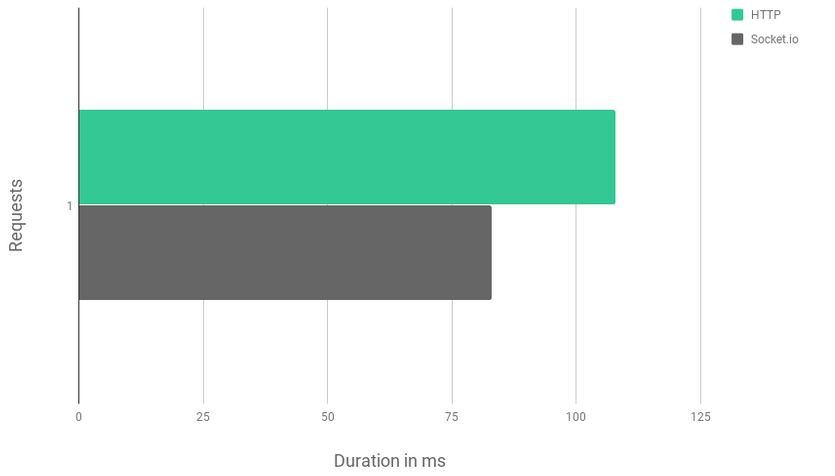
\includegraphics[width=0.5\textwidth]{Command_SocketvsHTTP_1.JPG}\label{fig:f1}}
    \hfill
    \subfloat[Data transfer for actual requests]{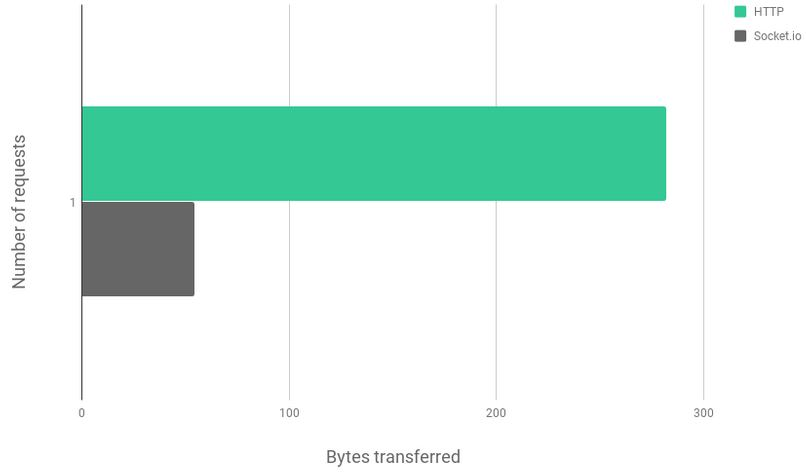
\includegraphics[width=0.5\textwidth]{Command_SocketvsHTTP_2.JPG}\label{fig:f2}}
    \caption{Comparison of HTTP and Websocket protocols \cite{SocketvsHTTP}}
\end{figure}

\subsubsection{Frontend}

The website of the Command module was created with React which is a JavaScript library that combined the speed of JavaScript with more easier method of rendering webpages that are highly dynamic and responsive to user input. Due to its component design, it naturally compliments the project's Modularity and Scalabity design theme. React is well-documented which made it easier for beginners to start developing quickly.    

\begin{figure} [h!]
    \centering
    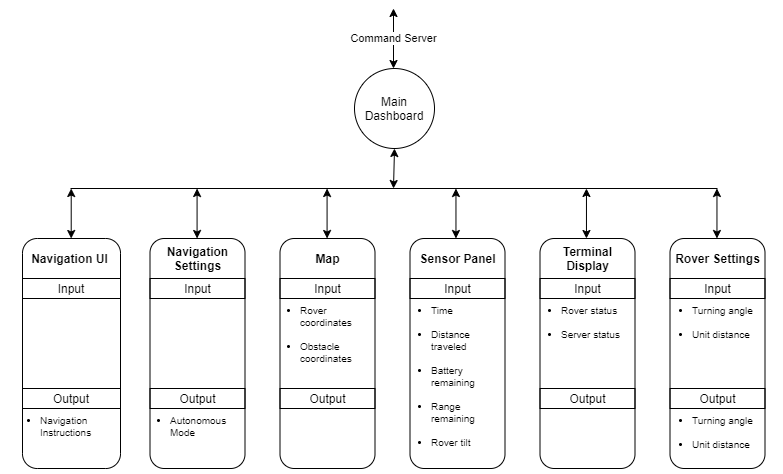
\includegraphics[scale=0.5]{Command_Frontend.png}
    \caption{Frontend functional diagram }
\end{figure}

Due to the frontend being the point at which the user interacts with the rover system, UI and UX design factors were important factors of consideration in addition to scalability. The website was custom built without any templates and used the wireframe method to model the website for team feedback before implementation. The following design choices were made with these taken into account:
\begin{itemize}
    \item \textbf{Simplicity}: The Command interface must be minimal, allowing the user to intuitivly interact with the system. All rover information and actions must be easily seen and not require users to navigate around to find the information they need.
    
    To meet this design choice, the website only has one page that is divided into six grids that each contain a component of the rover's command system such as the map and rover navigation interface. This one-page design meant users do not have to click around to find information. The user would log in using their credentials and immediately be able to see key rover details in one glance.

    \item \textbf{Scalability}: Due to the open-endedness of the project requirements, the exact number of features to implement was not known. In order to prevent the Command module from limiting the number of features the rover system has, the system must be designed to be able to scale and add new features easily. 
    
    Taking advantage of components in the React framework and the grid like design of the website, each grid was defined as a component which itself contains sub-components like buttons and display fields. This allows Command to easily add or modify components to enhance the website's features. For example, the map component was modified throughout the project timeline to include features like the animated rover icon that showed the direction the rover is facing and the gray pathway that showed the previous rover locations.  
    
\end{itemize}


\pagebreak
\subsubsection{Backend}

The Command server was implemented with the open source python-based FastAPI framework. The python language was an important feature as the team felt comfortable using Python due to its readable and extensive well-documented libraries. 

The main concern of using Python as the server language was the relatively slow performance when compared to such as C++ and JavaScript. However, with the addition of Starlette and Pydantic, FastAPI is on par with frameworks like NodeJS and Go. 

\begin{figure} [h!]
    \centering
    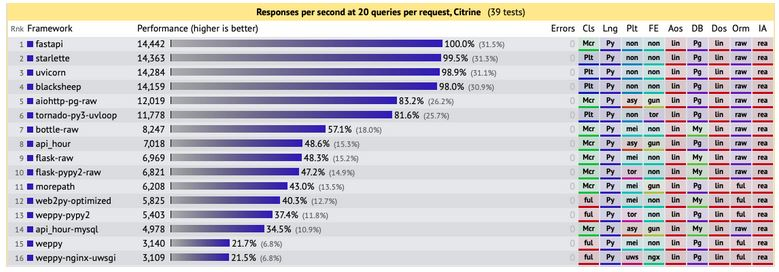
\includegraphics[scale=0.7]{Command_FastAPI.JPG}
    \caption{Benchmarks of framework performance \cite{FastAPI}}
\end{figure}

Being open-source, its interfaces are based on open standards for APIs which allowed easy connection to third-party services like authentication servers and databases. These features make the server design modular and scalable which was what the rover system required.  

\begin{figure} [h!]
    \centering
    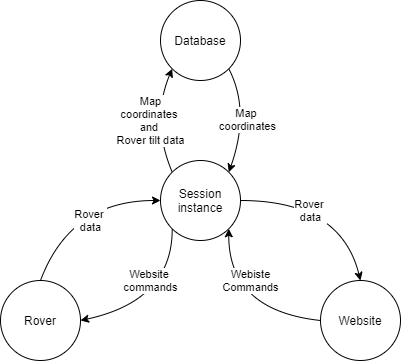
\includegraphics[scale=0.5]{Command_Backend.png}
    \caption{Backend context diagram }
\end{figure}

The function of the server was to basically act as a data hub that directs incoming data to the correct recepients. For example, all incoming data from the rover will be redirected to the website where it will be processed client-side. The only exception was map coordinates and the rover tilt measurements that are copied and redirected to the database component for storage.

\pagebreak
\subsubsection{Database}

The database component used MongoDB which is a NoSQL database. The design choice was based on the following advantages of MongoDB:
\begin{itemize}
    \item \textbf{Document-oriented}: MongoDB stores data in JSON-like objects and are non-relational. This allowed the Command module to store any records without having to specify a schema for the database. This meant any new features that generated new forms of data would not require modifications to the data-structure thus improving the system's scalabity potential.
    
    \item \textbf{Ease of use}: MongoDB is compatiable and well-documented on JavaScript and Python which is used in the Command module. in addition, MongoDB has an online intuitive database management system which helped in viewed the data stored in real-time.  
    
    \item \textbf{Mature ecosystem}: Developement can occur locally during testing and be easily ported into MongoDB Atlas which is a public server for deployment.
\end{itemize}

\subsubsection{Security}

Where users are concerned, the team believed that security needed to be incorporated into the design to prevent any unauthorised access to the rover system.

\begin{figure} [h!]
    \centering
    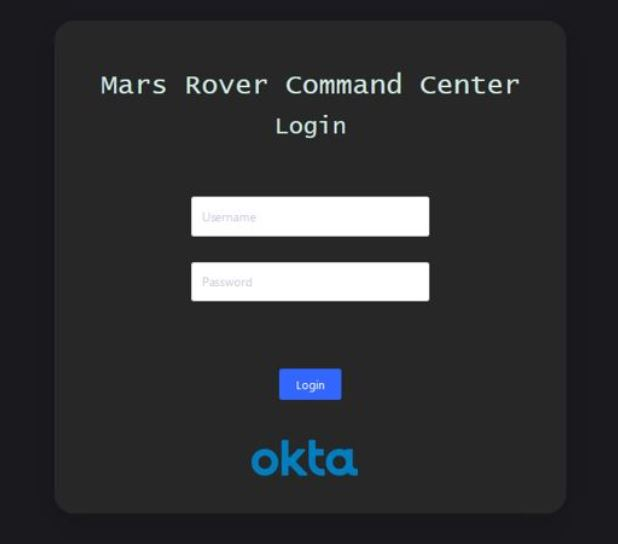
\includegraphics[scale=0.5]{Command_login.JPG}
\end{figure}

The Command module features a single-sign-on "Log In" page that prompted the user to authenticate themselves. The authentication system was implemented with Okta which provided an authentication server. Services like Okta are more secure than creating a custom authentication system especially with the constained project timeline. Any custom authentication system has the inherent security risks due to a rushed development and lack of expertise in such domain compared to a well-established like Okta. 

The design of the authentication system incorporating Okta is shown below:
\begin{figure}[!h]
    \centering
    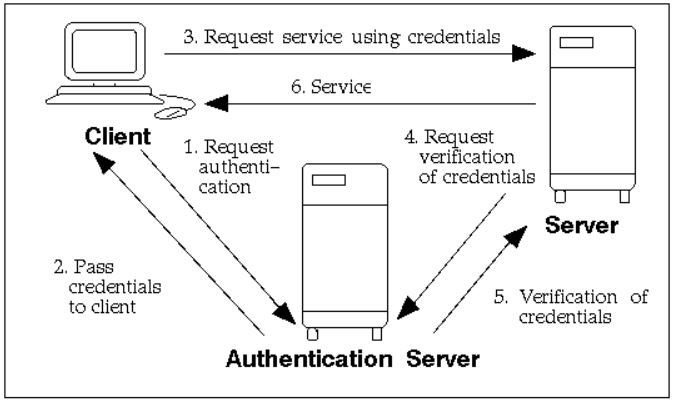
\includegraphics[scale=0.5]{Command_authen.JPG}
    \caption{Authentication system design \cite{Authentication}}
\end{figure}


\pagebreak

\subsection{Control}
%%%%%%%%%%%%%%%%%%%%%%%%%%%%%%%%%%%%%%%%%%%%%%%%%%%%%%%%%%%%%%%%%%%%%%%%%%%%%%%%%%%%%%%%%%%%%%%%%%%%%%%%%%

The Control module acts as a central data hub that passes the necessary data from other modules to the intended module. For example, the Drive module sends rover coordinates to the Command module.

\begin{figure} [h!]
    \centering
    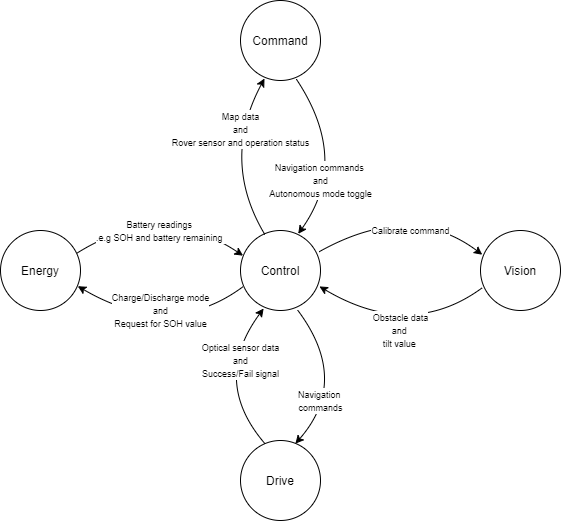
\includegraphics[scale=0.6]{Control_functional.png}
    \caption{Control module context diagrams}
\end{figure}

With the Arduino architecture, Command supports various interfaces. Each interface has advantages and disadvantages as summarised below:
\begin{figure} [h!]
    \centering
    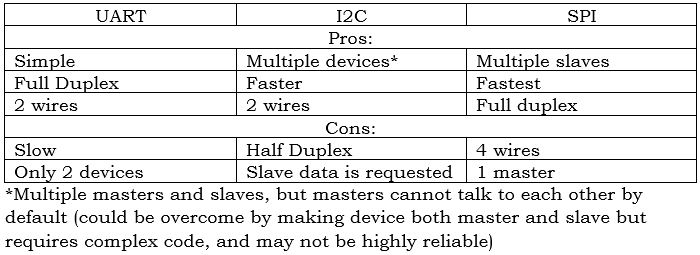
\includegraphics[scale=0.7]{Control_table.JPG}
\end{figure}

\subsubsection{Drive}

As the Mars rover was designed to operate in a remote location, the system was design to ensure the user knows when an instruction has failed to execute. In the Drive module, the Drive module sends a "Instruction Successful" signal to the Control module whenever an instruction finishes. In a situation the instruction failed to execute, like when the rover detects an obstacle, it will send an error message to be displayed on Command.

%%%%%%%%%%%%%%%%%%%%%%%%%%%%%%%%%%%%%%%%%%%%%%%%%%%%%%%%%%%%%%%%%%%%%%%%%%%%%%%%%%%%%%%%%%%%%%%%%%%%%%%%%%
\pagebreak
\subsection{Vision}
%%%%%%%%%%%%%%%%%%%%%%%%%%%%%%%%%%%%%%%%%%%%%%%%%%%%%%%%%%%%%%%%%%%%%%%%%%%%%%%%%%%%%%%%%%%%%%%%%%%%%%%%%%

In additional the the functional requirements stated in the Project Management section, the Vision module has the following non-function requirements that helped enhance the rover system:
\begin{enumerate}
    \item Collect the position and colour of balls provided that:
    \begin{itemize}
        \item Distance between ball and rover was within $20$ cm - $80$ cm
        \item The ball does not touch the edges of the frame
        \item Rover inclination angle was less than $45$ degrees
        \item Rover operates under natural sunlight conditions
    \end{itemize}

    \item Balls can be detected but data cannot be recorded if the ball was within:
    \begin{itemize}
        \item Distance between ball and rover was greater than $14$ cm
        \item Rover inclination angle was smaller than $50$ degrees
    \end{itemize}

    \item Automatic gain and exposure calibration to adapt to different light levels.
    \item Accelerometer used to calculate inclination of rover.
\end{enumerate}

\subsubsection{Ball detection algorithm}

\begin{figure}[ht]
    \begin{minipage}[t]{0.5\linewidth}
    \centering
    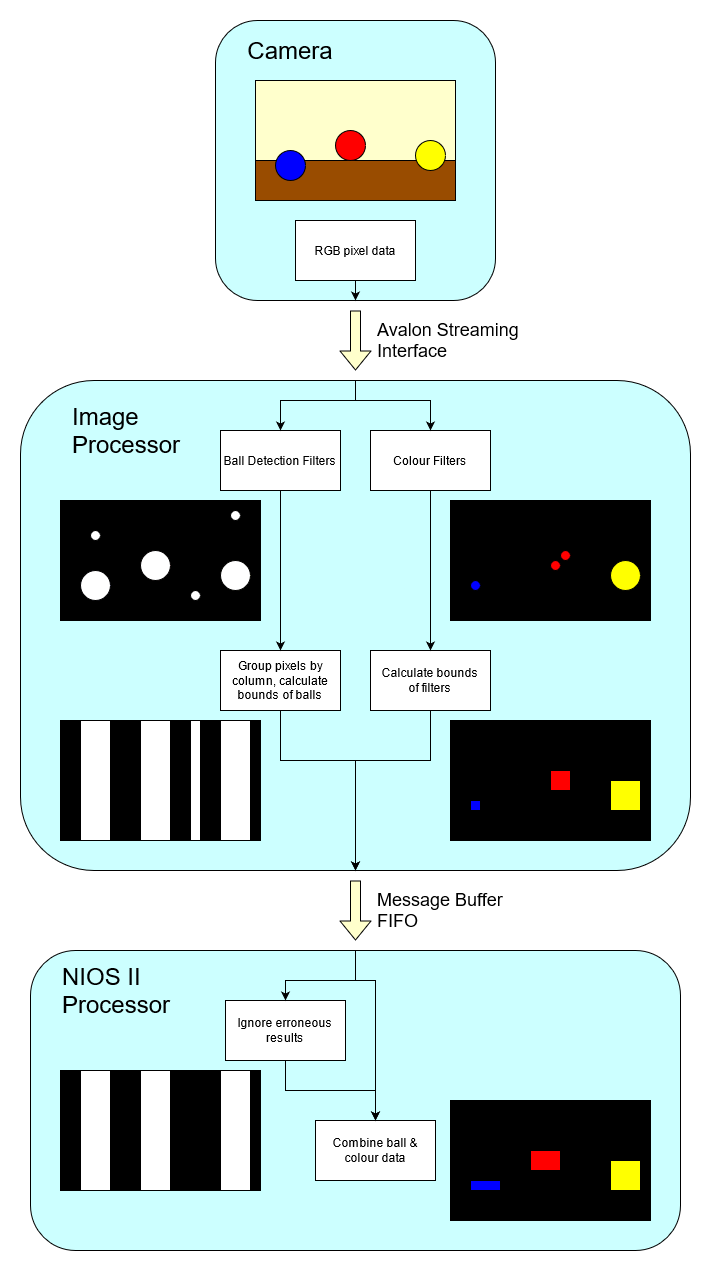
\includegraphics[%scale=1
                     width=0.9\linewidth, valign=t]{Vision diagram.png}
    \caption{Vision module functional diagram}
    \label{GIS_Mapping_Software}
    \end{minipage}%
    \begin{minipage}[t]{0.5\linewidth}
        The image processor receives a stream of RGB pixel values from the camera which could have been converted to HSV format. However, RGB format was used rather than HSV format because the hue varied greatly with different lighting conditions, which led to poor ball detection and obstacle avoidance. Using HSV format would have also required single cycle division in hardware, which would be expensive in terms of chip area.
        \\
        The image processor used filters to determine whether a given pixel could belong to a ball or not. There are two sets of these filters:
        \begin{itemize}
            \item Ball detection filters: Designed to reduce the reporting of false negatives, across a wide range of lighting conditions but provides no data about colour.
            \item Colour filters: This set has five filters, one for each ball colour. The colour filters have a very low chance of reporting false positives under sunlight, but they are very inaccurate under other lighting conditions.
        \end{itemize}
        
        The NIOS II processor remove erroneous data from the detected balls, then compare the data with the bounds of the colour filters, this give the positions and colours of all visible balls. 
    \end{minipage}
\end{figure}

If a ball was in the path of the rover while rover is currently moving, a signal will be transmitted over UART to stop the Drive module and send data of the blocking ball to Control. Otherwise, if a new ball was visible, but has not been seen before, its data will be transmitted to the command subsystem.

\subsubsection{Rover inclination calculation}

The accelerometer data was transmitted to the NIOS II processor over SPI, the y-axis and z-axis readings are used to calculate the inclination angle of the rover. This required the $arctan$ function, a fixed point approximation was created for this using the first three terms of the Taylor series. This approximation is only accurate for inclination between $\pm 20$ degrees:
\begin{gather*}
    a = \frac{y}{z} \\
    \arctan(a) \approx 56a - 16a^3 + 8a^5
\end{gather*}

\subsubsection{Testing conditions}

The testing conditions during the development of the Vision module are as follows:
\begin{itemize}
    \item Tested under sunlight (approximately 6500K) and 3000K 5W LED lamp:
    \begin{itemize}
        \item Varied brightness by varying distance to lamp or closing blinds partially.
        \item Varied direction of lamp and sunlight by rotating Vision camera and balls.
    \end{itemize}
    \item Background was a matte painted wall with wooden floor.
\end{itemize} 

\subsubsection{Calibration}

The gain and exposure could automatically adjusted when there are no balls in the field of view. The calibration system first sets both parameters to their maximum value, then reduces them until none of the colour filters are triggered and no balls are detected. This calibration process could be triggered remotely over UART.

\subsubsection{UART interface}

The UART implementation has "acknowledgement" signals designed to ensure all messages are transmitted successfully. The UART implementation also uses a ‘loose’ handshake protocol when transmitting data i.e. processor can process data, rather than idle, when waiting for responses. This was chosen over a ‘firm’ handshake because this method is much more resilient against errant characters or missing characters in transmission which has been detected during testing.



The UART interface transmits the following information to the Control module in the following events:
\begin{itemize}
    \item If there was a ball within 30 cm range of the camera view, an emergency stop signal was sent to the Control module.
    \item If a new ball had been detected, the "Pause" signal was sent to Control which was redirected to Drive in order to gather data.
    \item Ball data such as obstacle coordinates and ball color was transmitted after pausing the Drive module. If an emergency stop has been occurred, the first batch of data describes the particular obstacle causing the emergency stop.
    \item If no new ball data was left to transmit, a Continue signal was transmitted. This enables Drive to continue moving, or in the case of an emergency stop, informs Command that a ball was in the path of the rover.
\end{itemize}

\subsubsection{FPGA resource utilisation}

\begin{verbatim}
Flow Status	Successful                  Tue Jun 15 15:37:23 2021
Quartus Prime Version:                  16.0.0 Build 211 04/27/2016 SJ Lite Edition
Revision Name:                          DE10_LITE_D8M_VIP
Top-level Entity Name:                  DE10_LITE_D8M_VIP
Family:                                 MAX 10
Device:                                 10M50DAF484C7G
Timing Models:                          Final
Total logic elements:                   12,204 / 49,760 ( 25 % )
Total combinational functions:          10,595 / 49,760 ( 21 % )
Dedicated logic registers:              7,474 / 49,760 ( 15 % )
Total registers:                        7541
Total pins:                             171 / 360 ( 48 % )
Total virtual pins:                     0
Total memory bits:                      1,319,096 / 1,677,312 ( 79 % )
Embedded Multiplier 9-bit elements:     6 / 288 ( 2 % )
Total PLLs:                             1 / 4 ( 25 % )
UFM blocks:                             0 / 1 ( 0 % )
ADC blocks:                             0 / 2 ( 0 % )
Estimated Total logic elements:         13,020
Total combinational functions:          10569

Logic element usage by LUT inputs	
-- 4 input functions:                   5418
-- 3 input functions:                   2869
-- <=2 input functions:                 2282

Logic elements by mode	
-- normal mode:                         9093
-- arithmetic mode:                     1476

Total registers:                        7581
-- Dedicated logic registers:           7581
-- I/O registers:                       0

I/O pins:                               171
Total memory bits:                      1319096
Embedded Multiplier 9-bit elements:     6

Total PLLs	                            1
-- PLLs	                                1

Maximum fan-out:                        4232
Total fan-out:                          72189
Average fan-out:                        3.77
\end{verbatim}




%%%%%%%%%%%%%%%%%%%%%%%%%%%%%%%%%%%%%%%%%%%%%%%%%%%%%%%%%%%%%%%%%%%%%%%%%%%%%%%%%%%%%%%%%%%%%%%%%%%%%%%%%%
\pagebreak
\subsection{Drive}
%%%%%%%%%%%%%%%%%%%%%%%%%%%%%%%%%%%%%%%%%%%%%%%%%%%%%%%%%%%%%%%%%%%%%%%%%%%%%%%%%%%%%%%%%%%%%%%%%%%%%%%%%%
\subsubsection{Design}

\begin{figure} [h!]
    \centering
    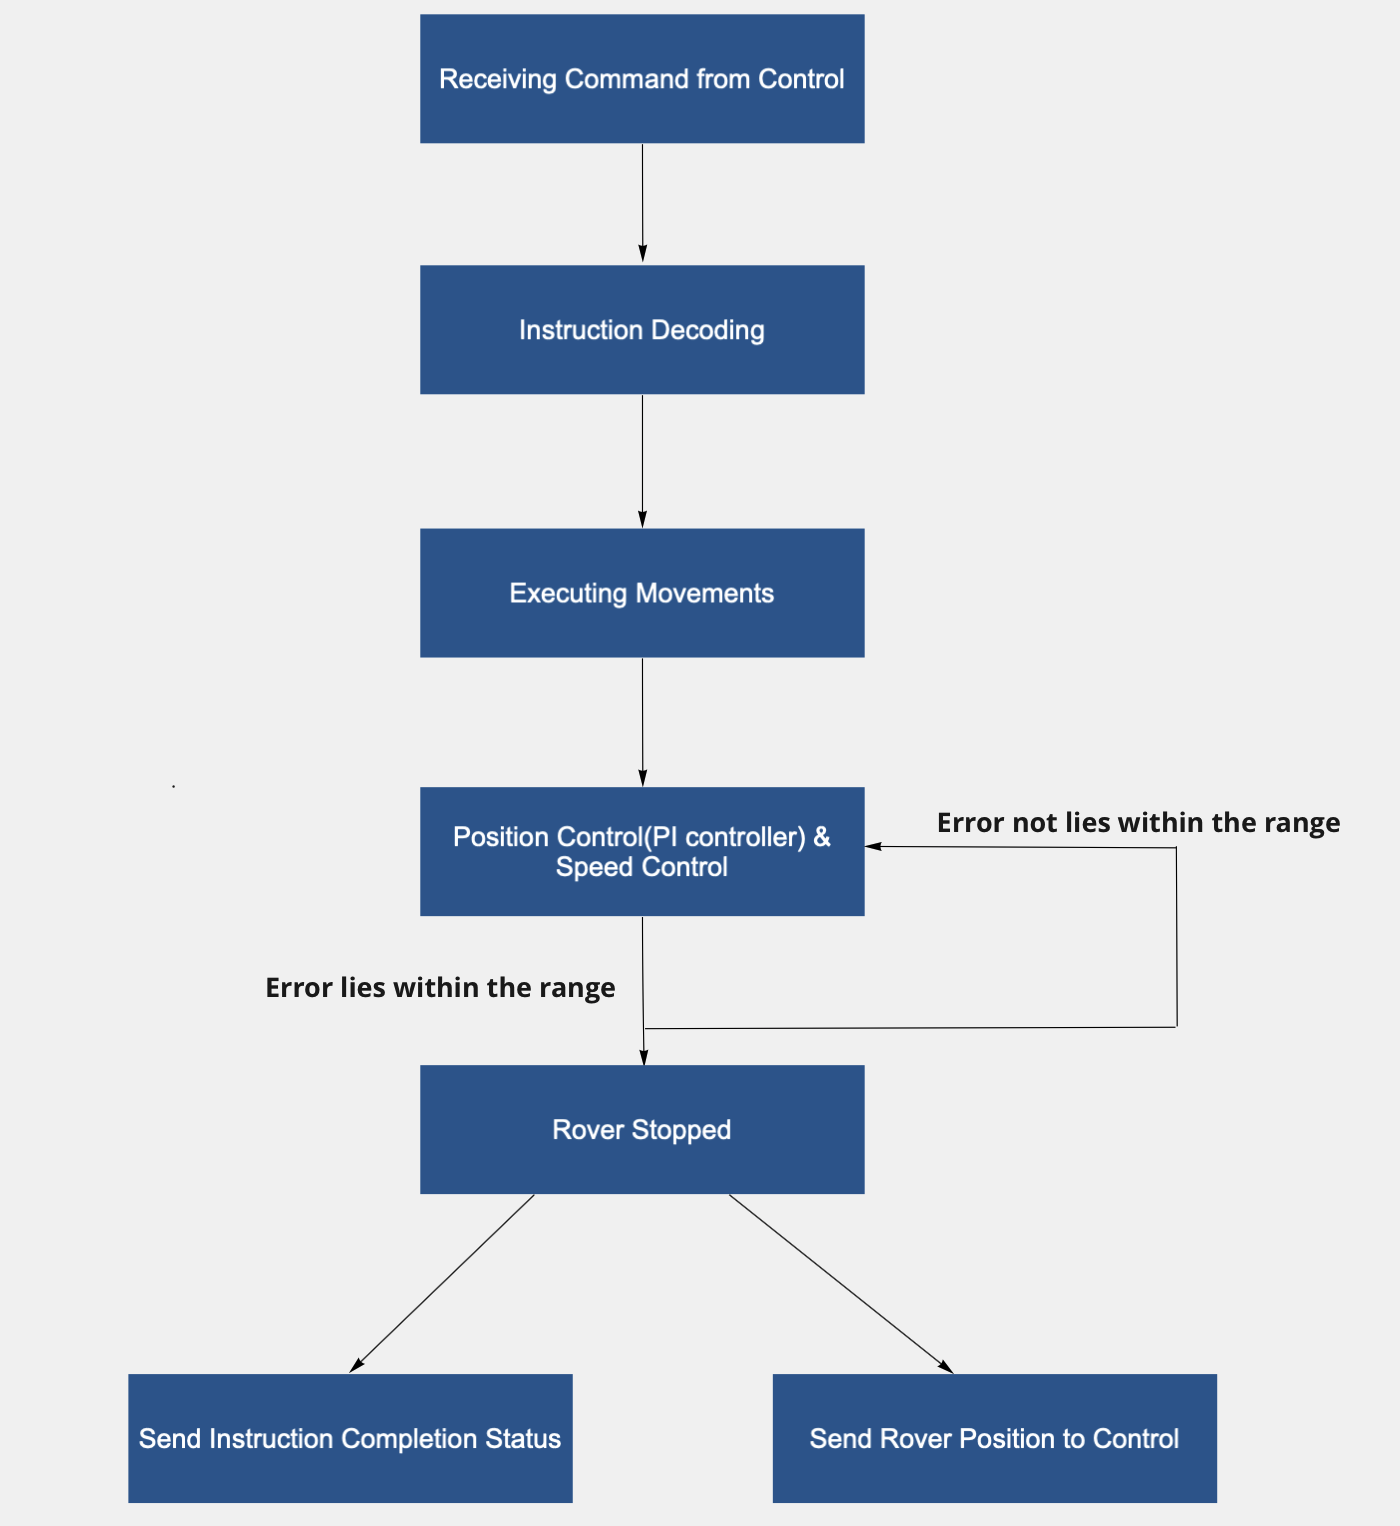
\includegraphics[scale=0.3]{Drive_functional.png}
    \caption{Drive functional diagram}
\end{figure}

The Drive receives nagivation instructions from the Control module and was designed to give user full control over the distance a rover goes per instruction and angle that the rover turns. The Drive instruction was defined as:
$$
\text{[Action]} + \text{[Turning angle]} + \text{[Distance]}
$$
where:
\begin{itemize}
    \item $\text{[Action]}$: Forward (F), Backward (B), Left (L), Right (R), Stop (S), Emergency stop (X)
    \item $\text{[Turning angle]}$ and $\text{[Distance]}$ defines the position and speed control mechanisms
\end{itemize}

The instruction decode structure is shown below:
\begin{lstlisting}
if(String(instruction[0]) == "F") { // Moving Forward
    F = true;
    target_x = 0;
    // Convert to target distance
    target_y = 100*(String(instruction[3]).toInt()) + 10*(String(instruction[4]).toInt()) + (String(instruction[5]).toInt()); 
    B = false;
    L = false;
    R = false;
    S = false;
    // Accumulate distance or angle
    tmp_x = total_x + target_x;
    tmp_y = total_y + target_y;
}
\end{lstlisting}

\subsubsection{Movement}

Through H-bridge circuit, the DC motors could support four main movement directions: Forward (F), Backward (B), Left (L), Right (R). 

Forward and backward movement was acheived by enabling the H-bridge, setting the PWM signals and the motor states. For example, the code below defines forward movement: 

\begin{lstlisting}
void MovingForward() {
    digitalWrite(pwmr, HIGH); // Setting right motor speed at maximum 
    digitalWrite(pwml, HIGH); // Setting left motor speed at maximum 
    // Set motor state 
    DIRRstate = LOW; // LOW - Forward, HIGH - Backward
    DIRLstate = HIGH; // HIGH - Forward, LOW - Backward
    digitalWrite(DIRR, DIRRstate); 
    digitalWrite(DIRL, DIRLstate); 
} 
\end{lstlisting}

Turning left and right was achieved by setting the respective wheel state to LOW. After turning, any distance change was in the x-direction and would equal the circumference defined by the rover's optical sensor. Turning angles were defined from the point where the circle's radius was the distance between the optical sensor to the midpoint along the rover shaft which was measured as 15 cm. It was detected that the two wheels do not output the same amount of power. This affected the turning angle calculations since the circle radius i.e. the distance between the optical sensor to the midpoint along the rover shaft was 12.7 cm and calculations had to be compensated as shown below:

\begin{lstlisting}
float Angle_Conversion(float target_angle) {
    return (target_angle/90)*28; // Convert input angle to distance along x-axis
} 
\end{lstlisting}

The halt instruction was implemented by disabling the H-bridge and set the PWM signal feeding into the left and right wheel pins to LOW.

\subsubsection{Position Control}

The rover's position control was implemented with a closed-loop PI controller which used the error margin between the current rover position and the previous rover position. The logic was that if the rover moved forwards and backwards by 20 cm and the optical sensor detected that the rover did not reverse 20 cm, the error margin would be the difference between the current rover position and the previous rover position.  

The controller was designed such that if the error margin was either in the range $-0.5 \text{ cm} < \text{error in } y < 0.5 \text{ cm}$ or $-0.2 \text{ cm}  < \text{error in } x < 0.2\text{ cm}  $, the controller would consider the difference insignificant and rover would stop. Otherwise, the rover would either keep executing the current instruction or perform the reverse movement until it was within the error margin. 

\begin{lstlisting}
if(F){ // Forward movement position control
    err_y = total_y - tmp_y; // Calculate error
    cp = pi_d(err_y);
    Speed_Control(min(abs(cp)*0.01+0.4), 0.7); // Using PI controller result to control speed

    // Position Control
    if(err_y < -0.5) { MovingForward(); }
    if(err_y > 0.5) { MovingBackward(); }

    if(err_y > -0.5 && err_y < 0.5) {
        // First time the error lies in the given range
        if (firstTime) {
            instructionCompleteTime=millis();
            firstTime=0; 
        } 

        // Check the motion after 10sec for position correction
        if(millis()-instructionCompleteTime > 10000 && !firstTime && !instructionCompleted) {
            Stop();
            instructionCompleted=1;
            Send_Instruction_Completed(total_y,1,'F');        
        }

        Stop();
    }       
}
\end{lstlisting}

The intial design for position control was a P controller which could acheive proportional controlling but the settling time is too long as a result of the steady-state error. By adding the I (Integral) controller, the steady-state error effect was mitigated. The best effect of the PI-controller was achieved by setting $K_p = 1$ and $K_i = 1$. Taking advantage of the closed-loop control strategy, position control and speed control were linked together to achieve more advanced features that are elaborated in the next section. 

As an additional feature of position control, Drive module returns a SUCCESS signal to the Control module once an instruction was sucessfully completed. After 20 seconds, if the instruction was still not completed, the Drive module will return a FAIL signal and stop the rover immediately to await further commands. These signals can be directed to the Command module to display the rover's movement status on the Terminal interface built into the Command website and, with the WebSocket connection, gives real-time feedback on the rover's Drive status.  

\subsubsection{Speed Control}

The speed control was achieved by using the the PWM signals as inputs into the SMPS board duty cycle to control the output voltage applied to the motors. The implementation of speed control is shown below:

\begin{lstlisting}
void Speed_Control(float duty){
    // Use duty cycle as argument to control voltage thus control speed
    analogWrite(6, (int)(255-duty*255)); 
}
\end{lstlisting}

By inputting the position error in either the $x$ or $y$ direction into the PI control function, its output was  inputted into the speed control function. After testing and caliberation, the duty cycle input function was determined as:
$$
    (\text{error from PI controller} \times 0.01) + 0.4
$$
where $0.4$ was the minimum voltage required to activate the rover. If the rover stays at a place for a long time,due to the presence of the integral controller, the error would accumulated as time increases and the speed control function will increase the rover speed to correct the error. Through testing, the rover initially accelerated due to a significant initial error. As the rover approached the target, the rover decelerated, indicating that the measurements taken by the optical sensor was more accurate. This method effectively reduced the number of oscillations and resulted in a more accurate Drive performance.

By using the formula: $\text{speed} = \frac{\text{distance travelled}}{\text{timestamp difference}}$, the relationship between the duty cycle and speed can be displayed as a look-up table as shown in Figure \ref{fig:duty}. This relationship formed the foundation of two advanced Drive features. By using the tilt data from the FPGA in the Vision component, the rover can detect when it is going up a slope and will increase the speed relative to when the rover is on a flat surface. In addition, Drive supports a power-saving mode where the duty would be fixed between 0.4 to 0.7 to conserve the energy used.

\pagebreak

\begin{figure} [h!]
    \centering
    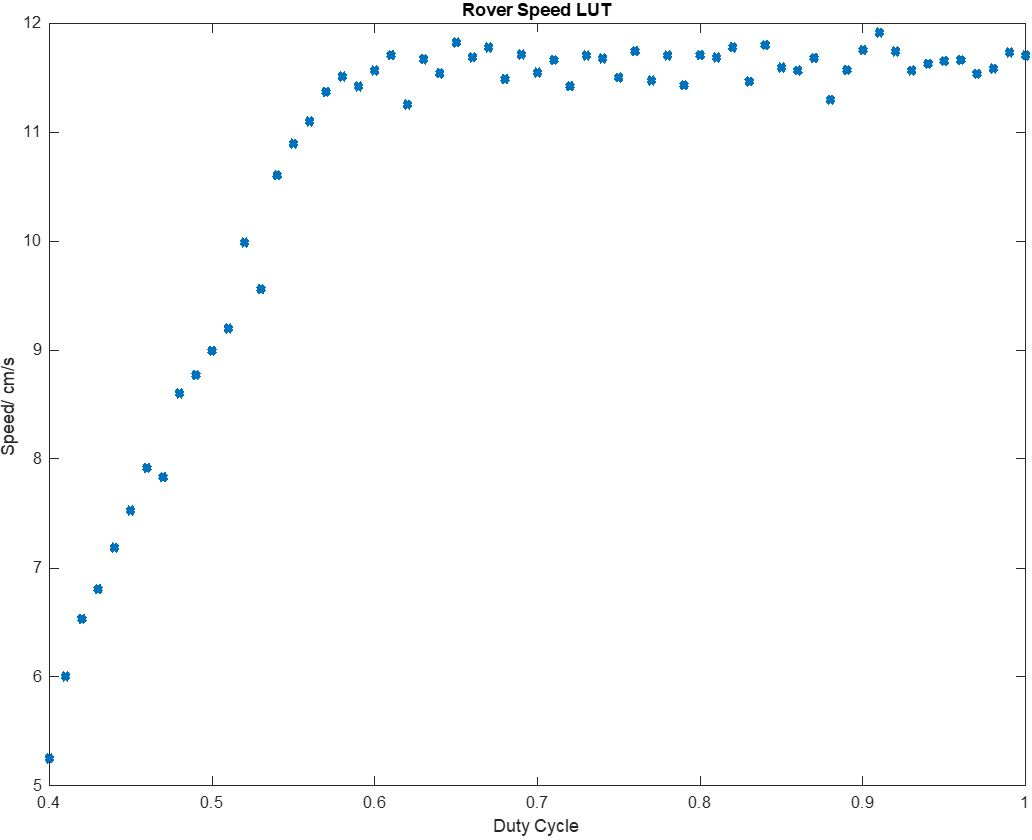
\includegraphics[scale=0.4]{Speed_duty_cycle.jpg}
    \caption{Relationship between the speed and duty cycle}
    \label{fig:duty}
\end{figure}



\subsubsection{Optical Sensor}

The optical sensor measures the distance of the rover travelled and the turning angle. To obtain more accurate measurements, the data type was changed from integer to float. The turning angle and travel distance was sent to the Control module for calculating the coordinates along $x$ and $y$ direction. The orientation was defined as:
\begin{itemize}
    \item The $y$-coordinate or $x$-coordinate changes positively if the rover faces North or East respectively.
    \item The $y$-coordinate or $x$-coordinate changes negatively if the rover faces South or West respectively.
\end{itemize}

\subsubsection{Advanced features}

The Vision module is able to directly issue commands to the Drive module through the Control module. Vision module issues three commands: Pause (P), Next coordinate (N) and Unpause (U). This was implemented to allow the Vision module to stop the rover if it detected an obstacle like a ball or an object that could collide with the rover. During Pause, the rover will send the x-position of the rover. Once Control has received it, Control would send the N flag which Drive will send the y-position. After the Unpause command is issued, the rover would continue executing the current set of instructions \footnote{The implementation is attached in the Appendix: Drive module: Pause feature}.
    
"Emergency Stop" action (X) is issued by Vision when a ball is in the path of the rover and would collide if the rover did not stop. The "Emergency Stop" is different from the standard "Stop" where if the "Emergency Stop" was used, the rover status will be updated to display an error has occured which is not the case for the standard "Stop" action. 


\vfill
%%%%%%%%%%%%%%%%%%%%%%%%%%%%%%%%%%%%%%%%%%%%%%%%%%%%%%%%%%%%%%%%%%%%%%%%%%%%%%%%%%%%%%%%%%%%%%%%%%%%%%%%%%
\pagebreak
\subsection{Energy}
%%%%%%%%%%%%%%%%%%%%%%%%%%%%%%%%%%%%%%%%%%%%%%%%%%%%%%%%%%%%%%%%%%%%%%%%%%%%%%%%%%%%%%%%%%%%%%%%%%%%%%%%%%
\subsubsection{Battery Charge Profile Design}

A battery charging profile ensures that the cells are charged to their full capabilities while within the constraints of the batteries which was max $3.6$ V and min $2.4$ for the battery. The capacity of the cells were determined by the following formula before developing the battery charging profile:
$$
\text{Cell capacity} = \frac{\text{Discharging state time}}{3600} \times \text{current}
$$

The Energy module developed its own charging code that used a combination of Constant Current (CC) and Constant Voltage (CV) instead of the original method in the provided code which only used Constant Current to charge the cells. Constant Current was used when the cell was nearly empty to prevent overheating during charging\cite{Energy_constant_current}. When the battery has been charged to $3500$ mV i.e. around 90\%, Constant Voltage was used to charge it to avoid overcharging. 

The cell capacity measured by the provided standard code is $502$ mAh while the cell capacity value measured by the custom charging code was around $565.07$ mAh. This difference in measured cell capacity indicates that charging using a combination of Constant Voltage and Constant Current is more effective at fully charging the battery compared to using Constant Current only. The performance of the two charging methods over a period of time is shown below:
\begin{figure} [h!]
    \centering
    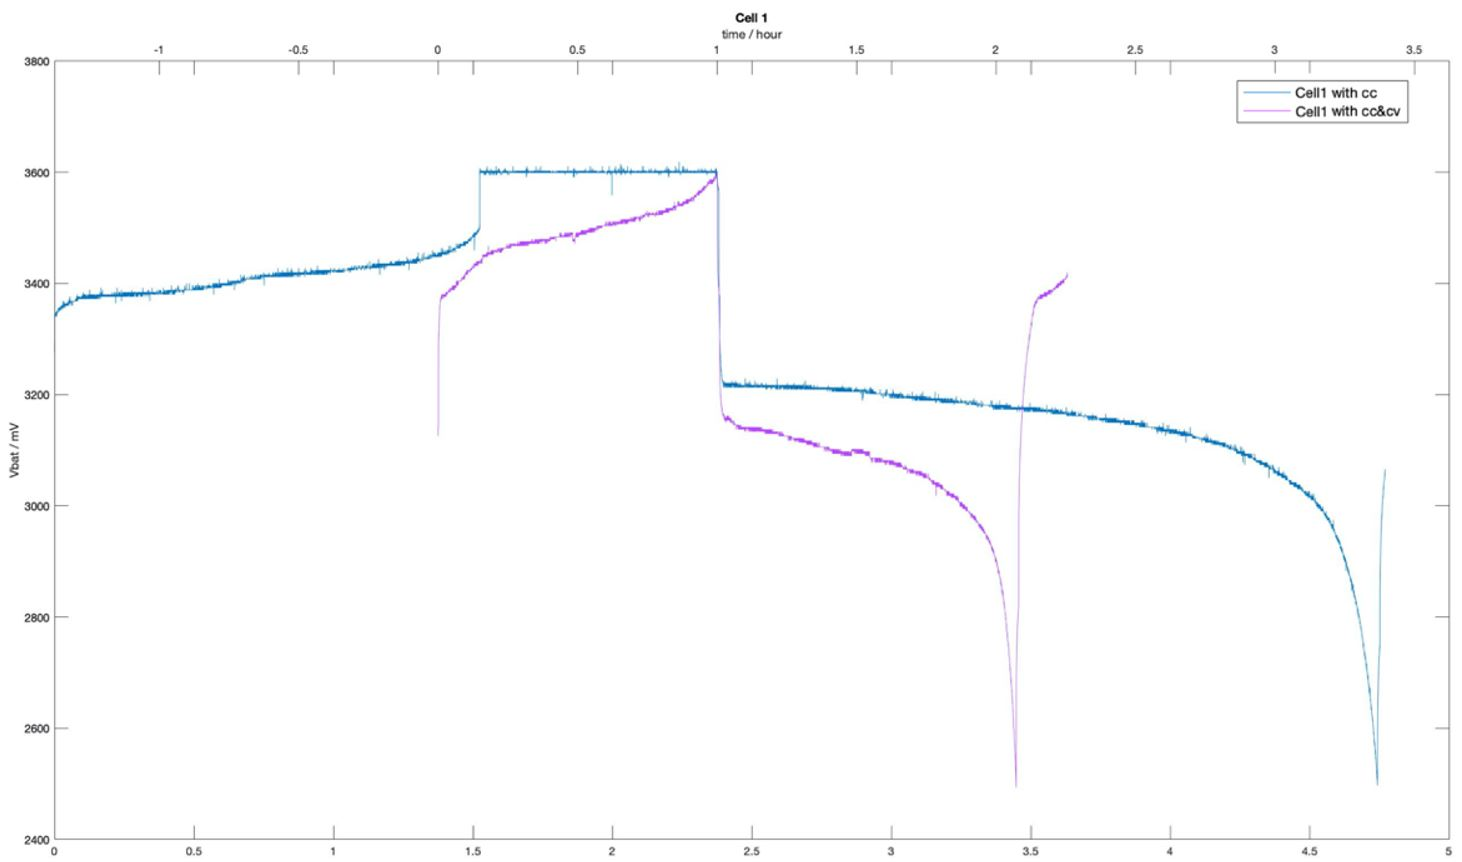
\includegraphics[scale=0.5]{CC and CV.JPG}
    \caption{CC vs CC + CV performance comparison}
\end{figure} 

\pagebreak

\subsubsection{Battery Balancing Algorithms}

The Energy module was design to use three cells connected in parallel. As a result, in addition to ensuring that each cell had a similar voltage at the start of the charging process, balancing was also required during the charging process. 

The balancing algorithm was design with $13$ states and Figure 4 shows the transitions between each states.    

\begin{figure} [h!]
    \centering
    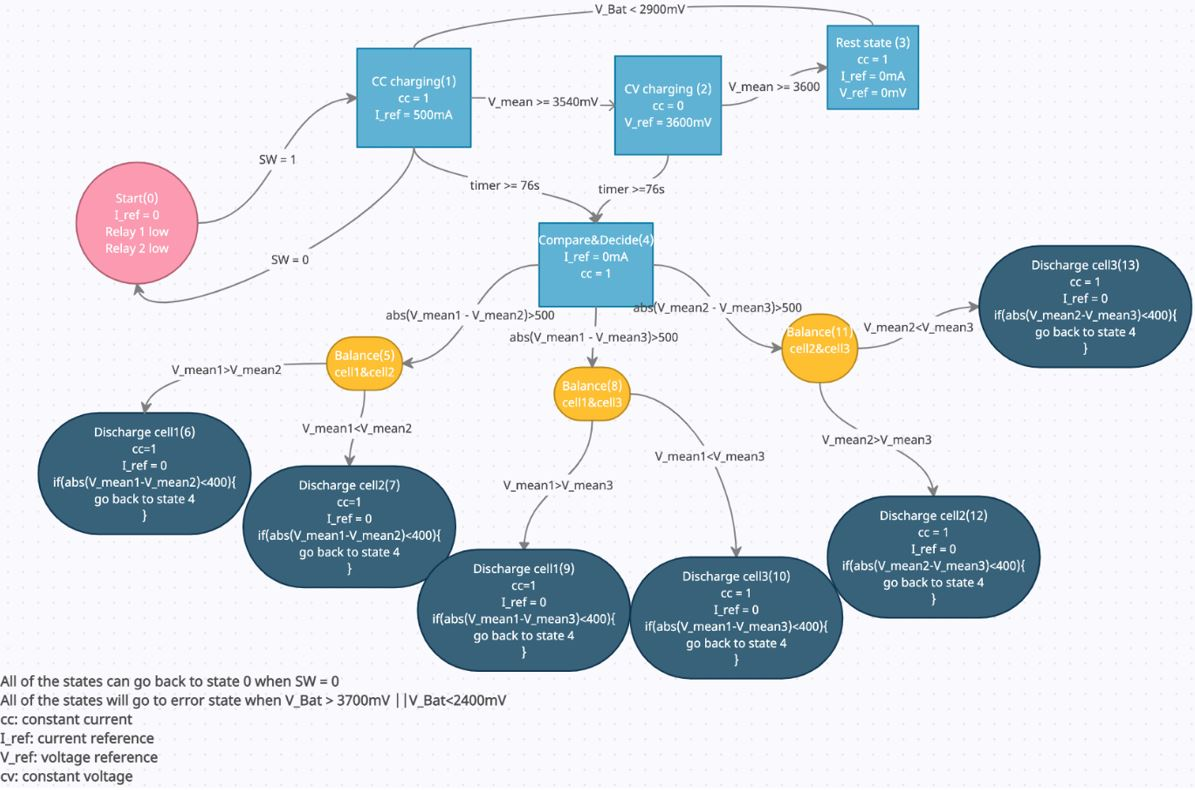
\includegraphics[scale=0.65]{Energy_state.JPG}
    \caption{Balancing Algorithm State Flow}
    \label{fig:State}
\end{figure}

For example, in the constant current charging state, the batteries are charged for 60 seconds and each cell was measured for 5 seconds respectively. The average value of each cell was then calculated and the state transition to the comparison state. In the comparison state, difference between the mean of two cells was compared. If it was greater than $500$ mV, the cells needed to be balanced and the higher-voltage cell would be discharged. The current state returns to state 4 after discharge to check if the difference between the other cell voltages was more than $500$ mV. The process repeats itself.

\pagebreak
\subsubsection{State of Charge}

The Energy module uses a combination of voltage lookup tables and coulomb counting to estimate the State of Charge. To obtain the voltage lookup table, a cell was completely charged and then discharged, the average value of the recorded cell voltage measured. To find the associated State of Charge at this voltage, the discharging process was stopped every 10 seconds and measurements taken.

The measured cell voltage from two different cells were plotted: 
\begin{figure}[h!]
    \centering
    \subfloat[\centering]{{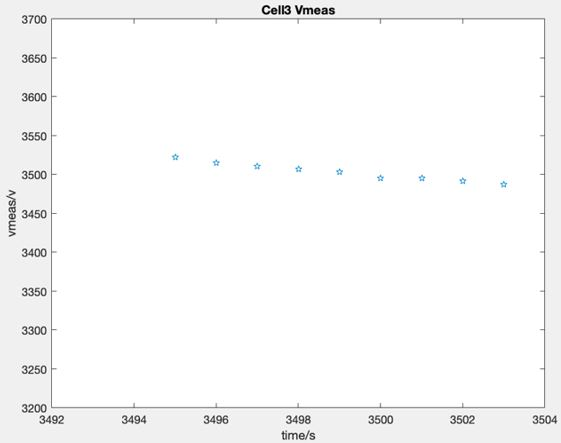
\includegraphics[width=7cm]{Energy_cell_v2.JPG} }}
    \qquad
    \subfloat[\centering]{{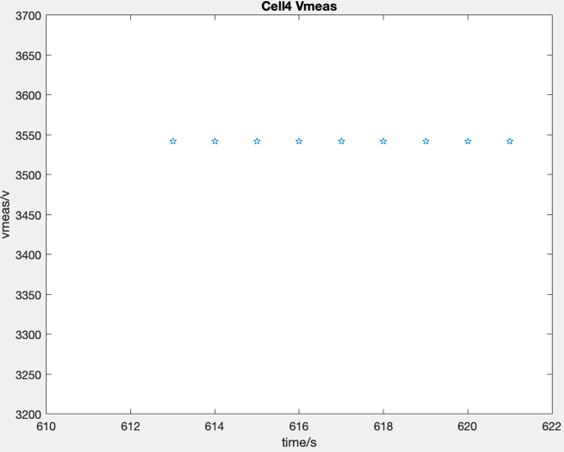
\includegraphics[width=7cm]{Energy_cell_v3.JPG} }}
    \caption{Cell voltage measurement}
    \label{fig:Cell}
\end{figure}


From Figure \ref{fig:Cell}, $3540$ mV was chosen since the average value of different cells in \textit{State 2} was approximately $3540$ mV. 

\begin{figure} [h!]
    \centering
    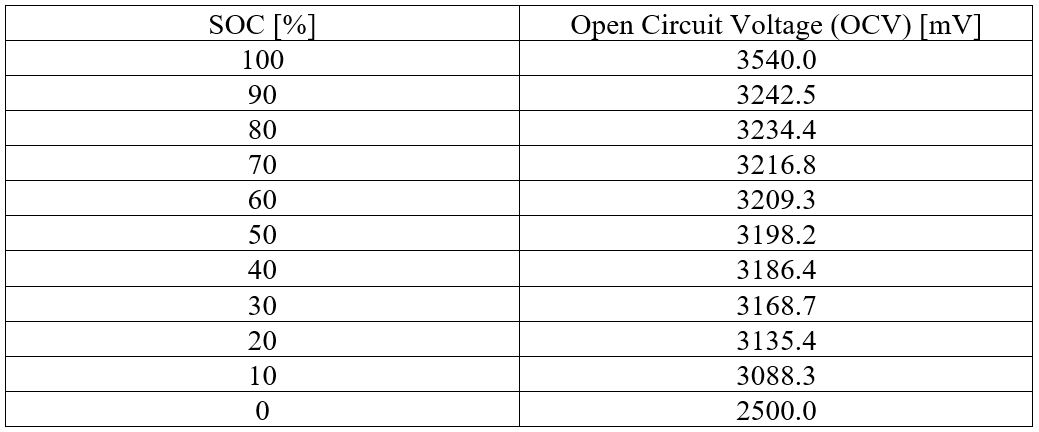
\includegraphics[scale=0.6]{Energy_SOC.JPG}
\end{figure}

Referring to the table, the OCV boundaries are not uniform. In the Energy module implementation, the boundaries between each OCV value was slightly modified to make the range more uniform. The algorithm always checks the value of the SOC before the start of the charging process.

The voltage lookup table was incorporated into \textit{State 0} in order to check the initial SOC value at the start of the charging process. During charging process, the SOC can be calculated by through the Coulomb Counting which measured the current drawn out of a cell and integrated the current over time in order to estimate the SOC:
$$
    \text{SOC} = \text{SOC} + \frac{\text{Measured current}}{\text{Cell capacity} \times 3600} \times 100\%
$$

\pagebreak

\subsubsection{PV MPPT Algorithms}

MPPT ensures that the PID controller does not encounter a problem when the PV voltage starts to fall where it will ask for more duty cycle. There would be no increase in current so the PID controller would repeat until the duty is maxed and the current is zero \cite{PV_MPPT}.  

In order to implement the MPPT, the PV panels would need to be characterised. The form of a PV cell's IV characteristic was determined to be that of a non-ideal current source \cite{PV_current} where the current decreases gradually at first and then rapidly as the voltage across the source rises.

The intended objective of the Energy module was to convert as much sunlight as possible into useable energy, hence the key design problem was where to operate on the IV characteristic that maximised the IV product. By characterising the PV panel, voltage with largest power can be identified. The PV panel was characterised by connecting different values of loads to buck and boost mode and measuring the current and voltage using a multimeter. From Figure \ref{fig:IV_char}, it can be seen that the voltage that provided the largest power was $4.7$ V.

\begin{figure} [h!]
    \centering
    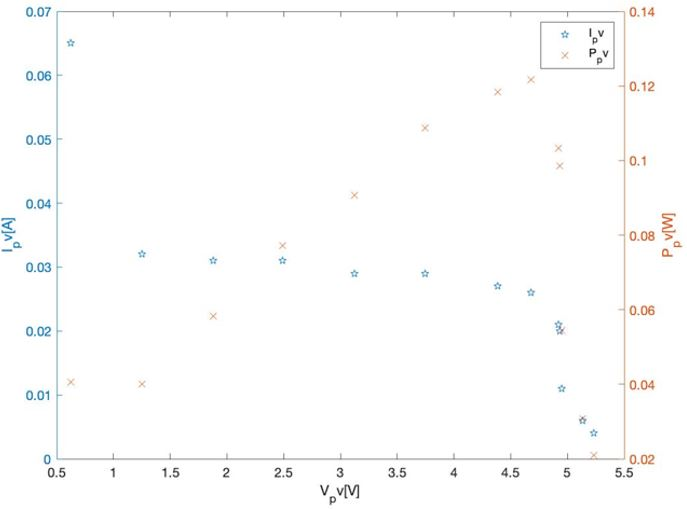
\includegraphics[scale=0.6]{Energy_PV_characteristic.JPG}
    \caption{PV IV characteristic}
    \label{fig:IV_char}
\end{figure}

The MPPT was designed and implemented with the Perturb and Observe Method \cite{PV_current}. This was due to the consideration that the intended use of the PV panels would be on the Mars rover and the IV characteristics of PV panels may vary in different environments. Therefore, the Energy module has incorporated a feedback system that maximises the value of the voltage output by using the fluctuating temperature and irradiance to determine the optimal operating point. The MPPT algorithm was implemented within the constant current component. If the measured current was smaller than $200$ mA, the algorithm will perform do MPPT. Otherwise, it perform constant current.

By using Perturb and Observe method, the maximum power point was found by comparing the present and previous power value, and varying the PWM accordingly. By varying the PWM, the resistance of the load changes, and the value of current and voltage change as well. By using the buck mode, if the present power was larger than the previous power, the PWM would be decreased by $0.005$. If the present power was smaller than the previous power, the PWM would be increased by $0.005$. A change of $0.005$ was selected because the value was a reasonably large enough range where the settling process of the values could be observed.

\pagebreak
\subsubsection{Circuit Design}

\begin{figure} [h!]
    \centering
    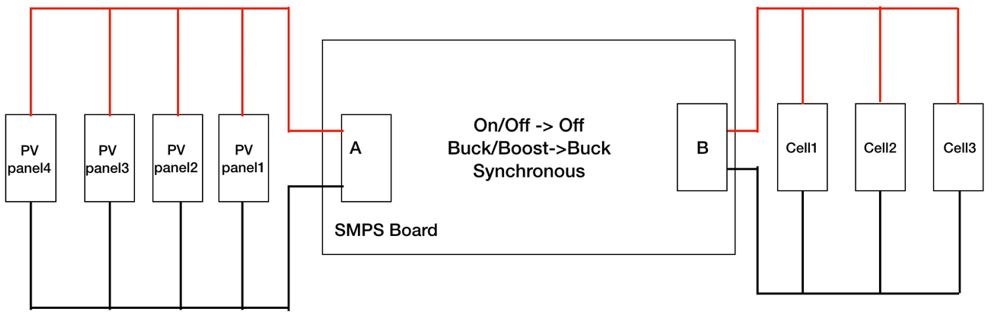
\includegraphics[scale=0.5]{Energy_parallel.JPG}
    \caption{Parallel cell design}
\end{figure}
The Energy module was design useing cells arranged in parallel. This was considered advantageous due to the following:
\begin{itemize}
    \item The whole energy system still operates even if one cell suffers an unexpected failure. The only effect to the Energy system would be an decrease in total cell capacity.
    \item Parallel cell arrangements also balance automatically provided that there was no significant difference between the voltage of all the cells before charging begins.
    \item The larger total current capacity of the system enables the system to function even on a cloudy day where PV panels are less efficient.
\end{itemize}

\subsubsection{State of Health}

The State of Health (SOH) is an indicator of the current condition of a cell compared to its ideal conditions. 
\begin{figure} [h!]
    \centering
    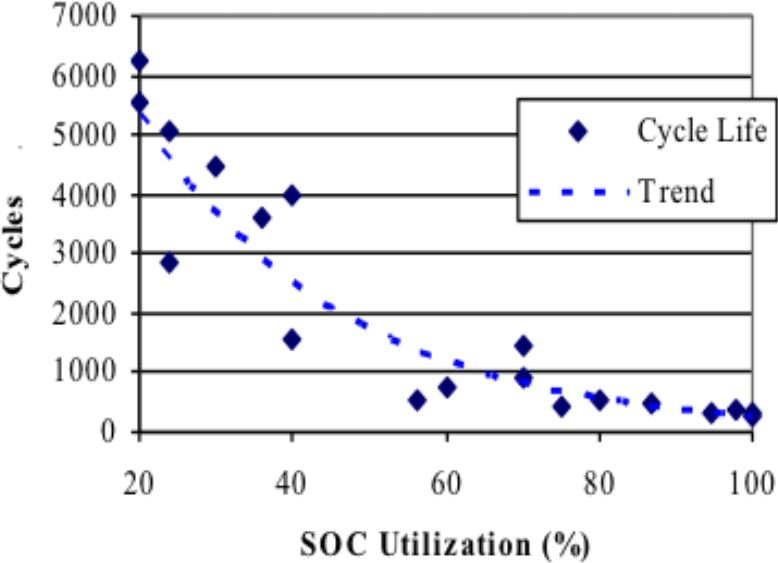
\includegraphics[scale=0.4]{Energy_SOH.JPG}
    \caption{Cycle life vs SOC use \cite{SOH}}
\end{figure}

Due to the time constaint of the project, it was not possible to charge and discharge the provided cells at least 400 times in order to plot the relationship between the SOH and the cycles. 

The Energy module has implemented several features to ensure the cells are kept as close to its ideal conditions during operation:
\begin{itemize}
    \item Overvoltage/undervoltage of each cell is consistently monitored by adding an error state for every single cell.
    \item The battery balancing algorithm implemented in the state machine ensures overcurrent does not occur.
\end{itemize}

The only concern that could not be mitigated was the battery temperature. A temperature sensor may be added to ensure the cell does not overheated for a long time.  

\pagebreak
\subsubsection{Energy to Control interface}

\begin{figure} [h!]
    \centering
    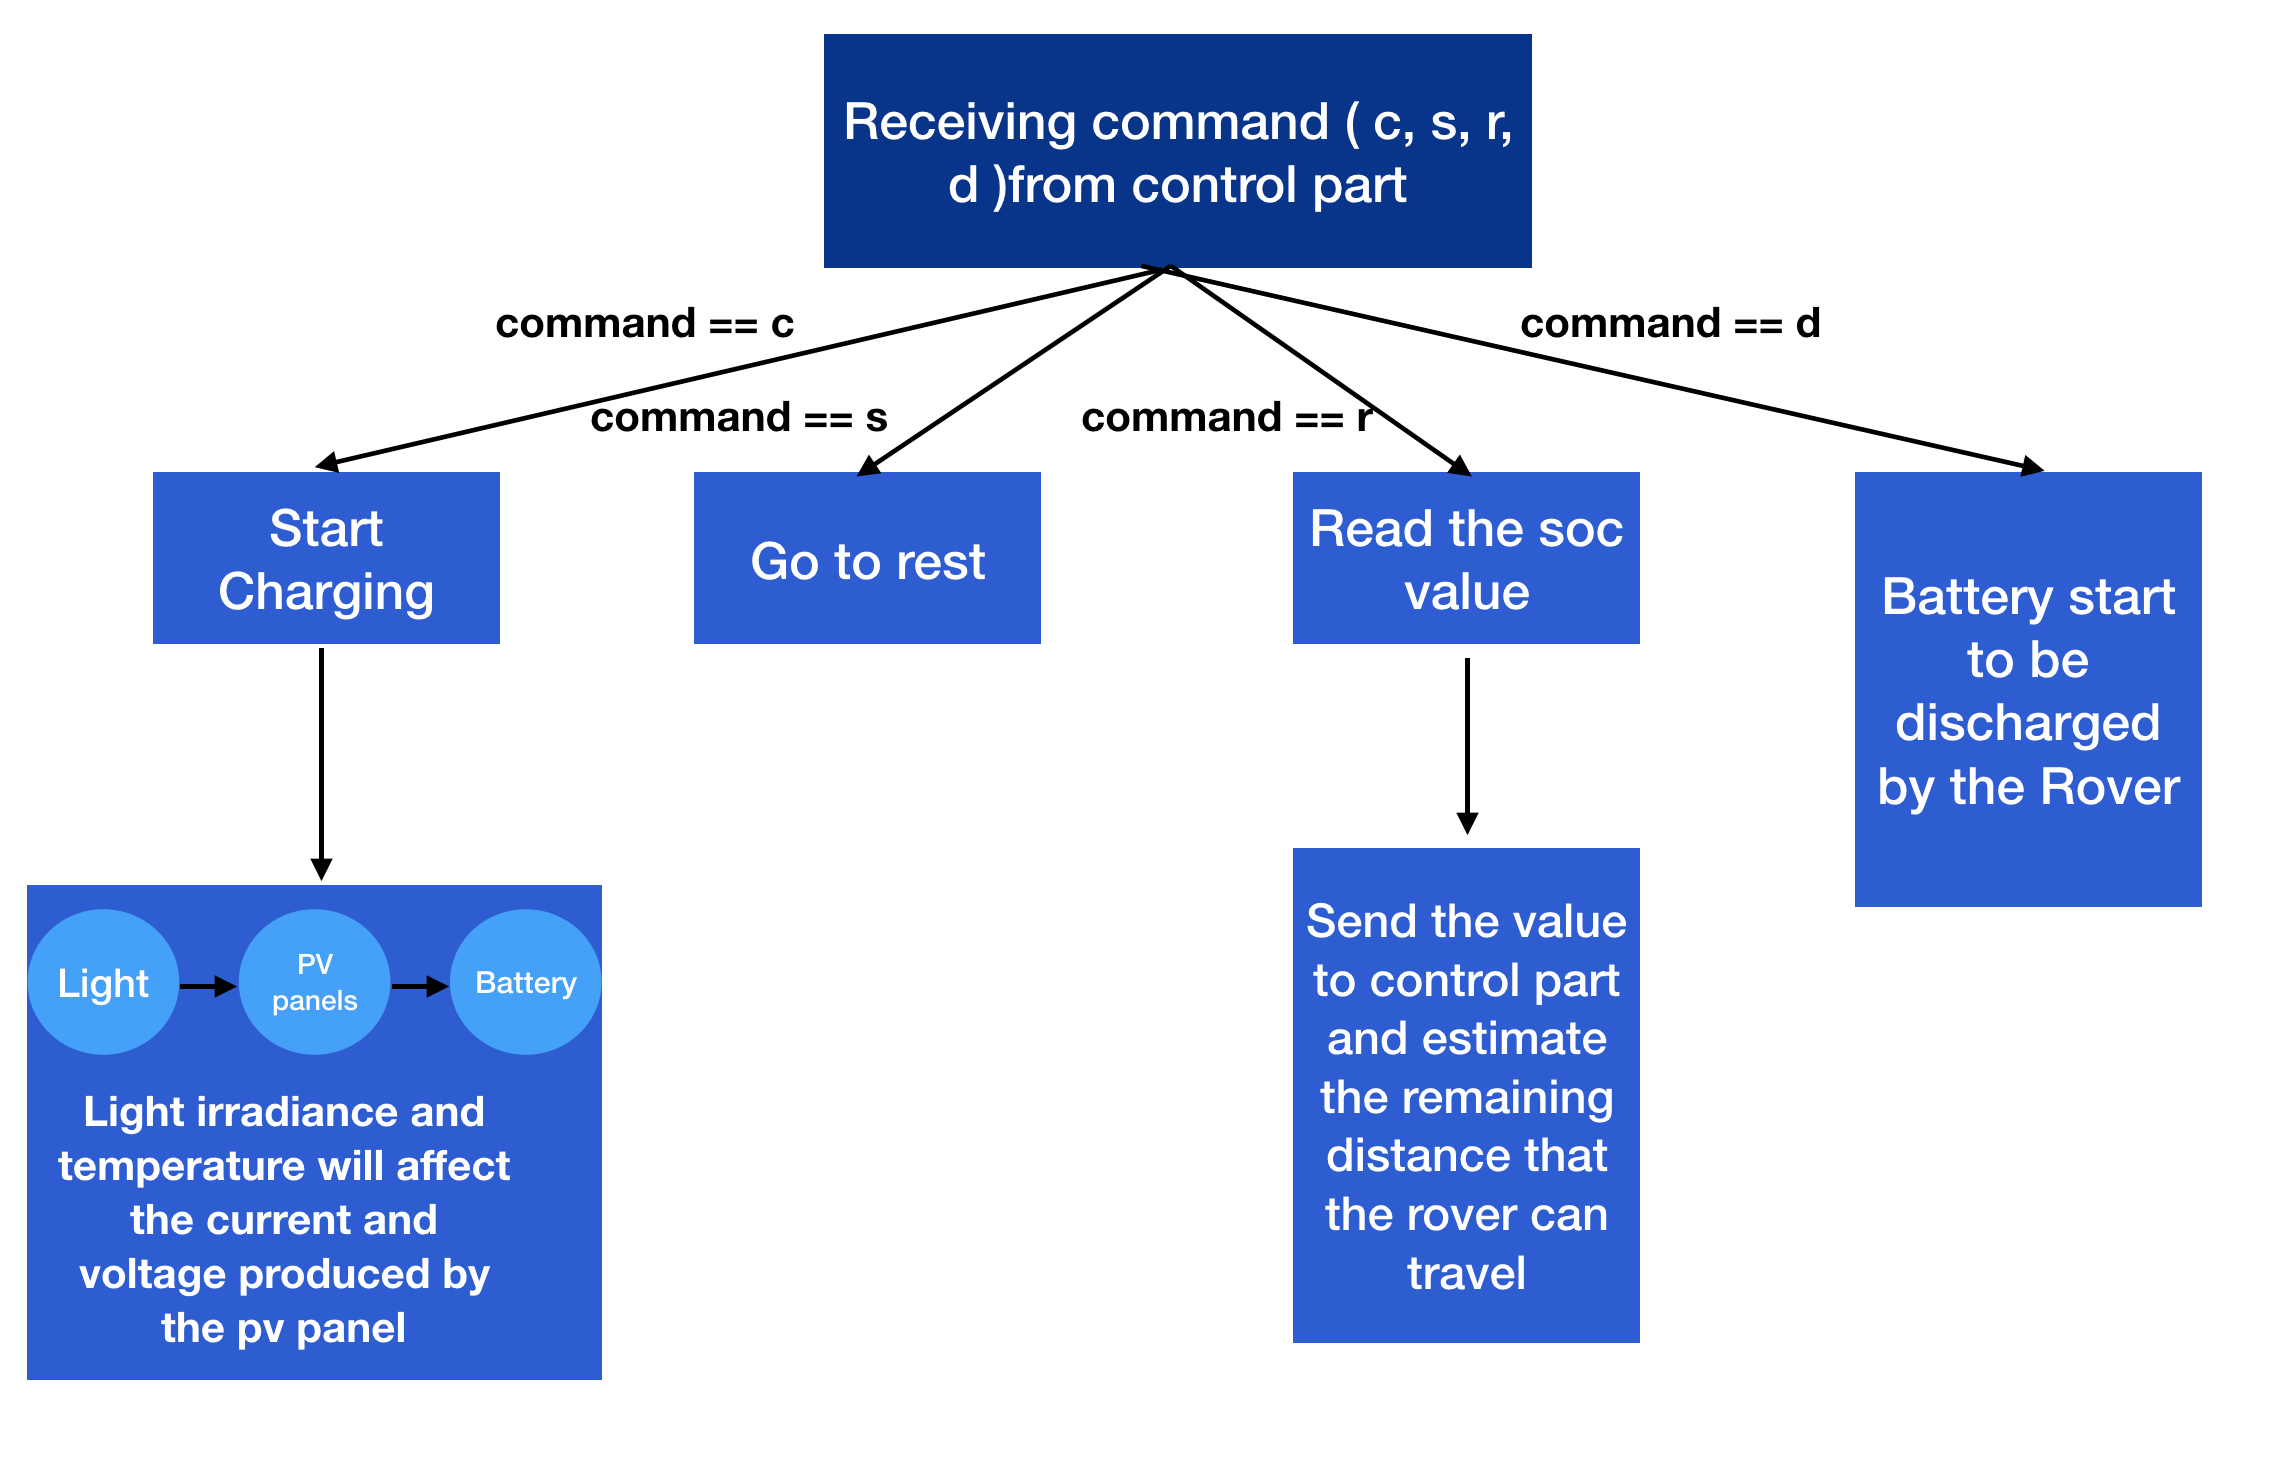
\includegraphics[scale=0.25]{Energy_functional.PNG}
    \caption{Energy module functional diagram}
\end{figure}

Energy module communicates to the Control module through the UART port:

\begin{lstlisting}
if(Serial.available()>0) {
    command = Serial.read();
    if (command == 'c') { // Read SOC value (state 0) and transition to charging state (state 1)
    state_num = 0;
    } else if(command == 'r') { // Read SOC value passes to the Command module
        Serial.println(soc); // Change to Serial1.print for communication with control sub module
    } else if(command == 's') { // Stop charging, go to rest state
        state_num = 3;
    } else if(command == 'd') { // Start discharge by the drive sub module
        state_num = 15;
    }
\end{lstlisting}

Because it cannot be tested with Drive module, the discharging process was imitated by a constant current mode with a reference current of 350 mA. 350mA was the value of the current that the Drive module uses while the rover was moving. To make sure all the cells have not been overvoltage/undervoltage, the battery should be balanced while discharging as well.

The Energy module passes the SOC value to the Control module which can be used to estimate the range that rover has left based on the battery remaining by using this equation:
\begin{gather*}
    \text{Time available} = \frac{\frac{\text{SOC value}}{100} \times \text{Total cell capacity}}{\text{Current drawn out}} \\
    \text{Range left} = \text{Time available} \times \text{Speed}
\end{gather*}
where "Total cell capacity" is defined as $565.07 + 543.68 + 554.51 = 1663.26$ mAh

A design problem in the Energy module was the location of the charging system. A static charging station could significantly reduce the weight of the Mars rover which would mean hgiher efficiency and simpler designs that leads to less possible points of failure. A charging station could include functionalities like additional sensors to monitor the health of the rover and replace failed parts like battery cells. 

Placing the PV panels on the rover would mean the rover's range is not constrained compared to if it has return to a charging station. The disadvantage, compared to the static charging station, would be the limited lifecycle of the battery cells and increase complexity of the rover. The Energy module chose to mount the PV panels since quality cell are sufficient and the advantages of not being constrained would be more important than the advantages offered by the static charging station.



\pagebreak
\section{Integration}

\subsection{Testing}

The Integration module was very reliant on the progress of other modules since its role was largely testing and debugging any errors. Every individual module was extensively tested before being combined with other modules to form more complicated systems. The only module that could not be fully tested was the Energy module due to Integration not having the hardware required. Only basic tests were performed since the Energy module used the Arduino Nano Every which the Drive module also used. 

The Integration module approached testing in the following phases: 
\begin{itemize}
    \item Stage 1: Each individual module 
    \item Stage 2:
    \begin{itemize}
        \item Command and Control 
        \item Vision and Control 
        \item Drive and Control
    \end{itemize}
    \item Stage 3: 
    \begin{itemize}
        \item Command to Control to Drive 
        \item Vision to Control to Drive
    \end{itemize}
    \item Stage 4: Full rover system test 
    \item Stage 5: Autonomous mode test 
\end{itemize}

\subsection{Drive}

Extensive testing was performed with the Drive module due to the low quality of the DC motors. The provided two DC motors were not outting the same amount of power due to a natural production variation. Due to the difference in value, its effects had to be considered and mitigated in the software in order to accurately calculate the rover coordinates. 

A further aspect that was discovered through testing was the weight of the rover. Any additional weights such as a powerbank to power the rover would cause the wheels of the DC motor to turn inwards which would cause the rover to not perform turns accurately. 

\subsection{Vision}
\subsubsection{Vision to Control Interface}
The connection of the Vision module to the Control module was one of the most complicated aspects of the project that required extensive testing and debugging to identify the error. Due to the lack of electrical lab equipment, the team could comprehensively test if the Vision fault was due to hardware like the FPGA board or software. 

Using a spare Arduino board, the team managed to convert the spare Arduino into an oscilloscope that allowed the team to check if the FPGA was transmitting any form of signal. 

\begin{figure}[!h]
    \centering
    \subfloat[Oscilloscope output showing electrical activities]{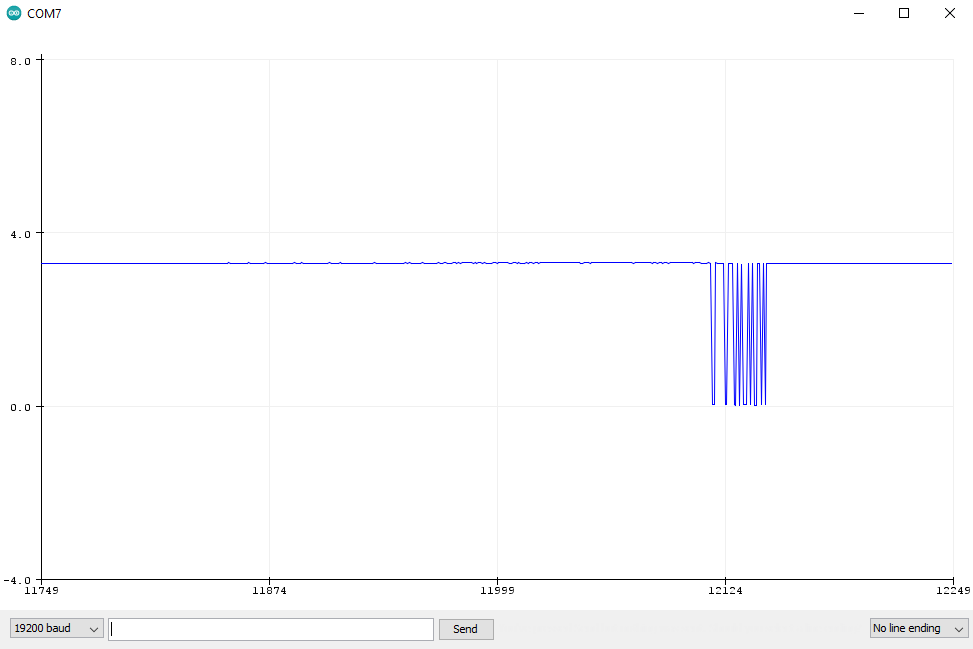
\includegraphics[width=0.5\textwidth]{Inte_Osci1.png}}
    \hfill
    \subfloat[Oscilloscope output showing no electrical activities]{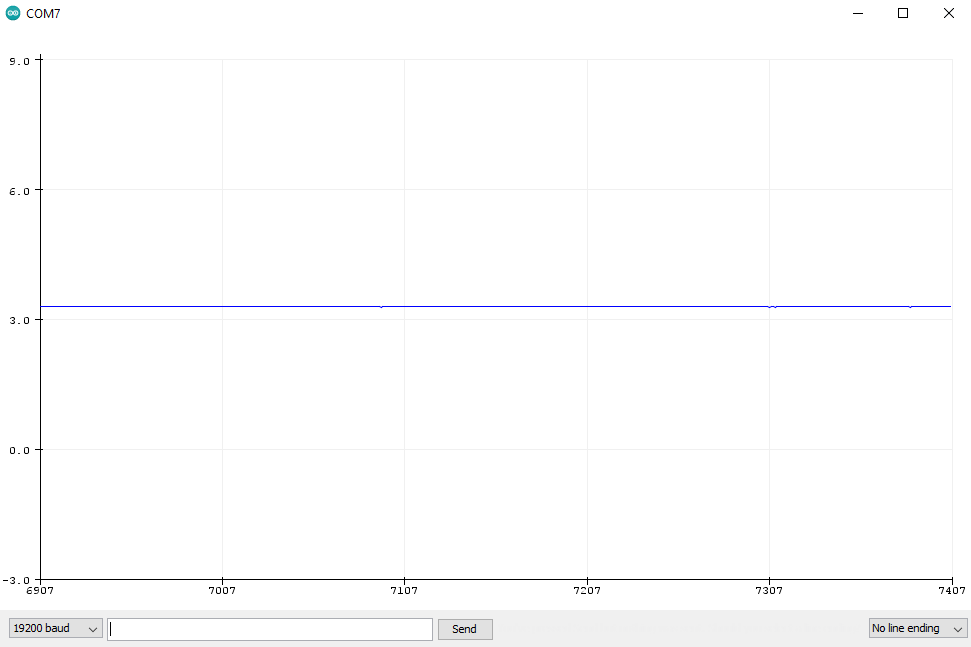
\includegraphics[width=0.5\textwidth]{Inte_Osci2.png}}
    \caption{}
\end{figure}

\pagebreak

The oscilloscope tool was implemented in Arduino code as shown below:
\begin{lstlisting}
    void setup() {
        Serial.begin(19200);
        pinMode(A0, INPUT);
    }

    void loop() {
        // Program code 
        Serial.println(analogRead(A0)*(5.0/1024.0));
        delay(7);
    }
\end{lstlisting}

\subsubsection{Ball recognition}

Through practical testing, the camera on the Vision module only recognises balls that are fully within its frame. If only part of the ball was in the frame, Vision would not be able to recognise it. This meant that, considering the height of the camera, Vision cannot recognise balls that are too close to the rover which risks the rover colliding with the obstacle. 

Vision has implemented a feature that detects obstacles that would collide with the rover and issue an "Emergency Stop" signal to Control which is the directed to Drive. This feature was fully implemented in the "main.c" file:
\begin{lstlisting}
if(ctrl_uart&&moving&&(!stop_ticks)&&((closest_distance<30)||(ball_bounds[3]>=472))){
    if(alt_up_rs232_get_available_space_in_write_FIFO(ctrl_uart)){
        alt_up_rs232_write_data(ctrl_uart, 's');
        stop_reasoned = 0;
        last_command = 's';
        stop_ticks = 9;
    }

    #ifdef VIEW_UART_MSGS
        printf("UART sent: s\n");
    #endif
    }

\end{lstlisting}

\pagebreak

\subsection{Energy}

In the Energy module, it was stated that the team opted to mount the PV panels on the Mars rover as this design choice was seen as more advantageous than the alternative which was a static charging station. The Integration module was tasked to research the best method to mount the PV panels and connect the system to the existing Mars rover interface. 

Having taken into account the current equipment provided to the project team, it was not possible to directly connect the Energy module to the Drive module. The Drive module was in Buck mode due to the requirement of having only voltages between $0$-$5$ V. The Energy module was using Buck mode due to the parallel cell connection design. However, in that situation, the voltage for Drive would constantly be fixed in the range of $2.4$ – $5$ V which meant the velocity range of the rover would be limited in the range as well.

There were two possible solutions proposed for this design problem:
\begin{itemize}
    \item \textbf{Relays}: Using two relays arranged in the following arrangement:
    \begin{figure} [h!]
        \centering
        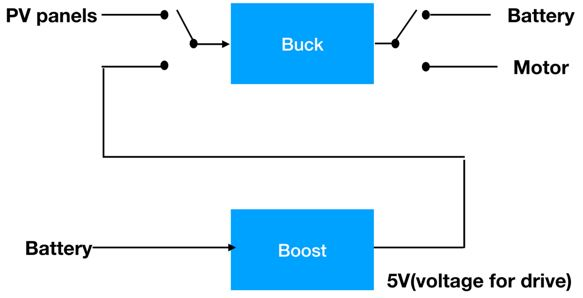
\includegraphics[scale=0.5]{Energy_int.JPG}
        \caption{Proposed two relay arrangement}
    \end{figure}

    When charging the battery, the relay on the left will be connected to the PV panels and the relay on the right will be connected to the battery. The Arduino Nano Every would be powered by the voltage produced by the PV panels by adding a regulator to make sure the Arduino was powered with $5$ V.

    When the rover moves, the relay on the left will be connected to Boost and the relay on the right will be connected to the Motor. The motor will be powered by the battery. However, the voltage across the battery decreases while discharging. Therefore, to make sure the output voltage of the battery was always at $5$ V, a PID controller can be added in the Arduino Nano Every on Boost to ensure the output voltage was fixed at $5$ V.
    
    \item \textbf{Add a third SMPS}: The second option would be to simply boost the output voltage of battery to $5$ V. But the drawback is that SMPS is more expensive than a relay.
    \begin{figure} [h!]
        \centering
        
\includegraphics[scale=0.6]{Energy_int2.JPG}
        \caption{Proposed additional SMPS arrangement}
    \end{figure}
    
\end{itemize}

The second option was chosen as the most preffered option since the SMPS, though more costly, was more efficient than the relay. Increased efficieny was seen as more important than increased cost of development.

%%%%%%%%%%%%%%%%%%%%%%%%%%%%%%%%%%%%%%%%%%%%%%%%%%%%%%%%%%%%%%%%%%%%%%%%%%%%%%%%%%%%%%%%%%%%%%%%%%%%%%%%%%
\pagebreak
%%%%%%%%%%%%%%%%%%%%%%%%%%%%%%%%%%%%%%%%%%%%%%%%%%%%%%%%%%%%%%%%%%%%%%%%%%%%%%%%%%%%%%%%%%%%%%%%%%%%%%%%%%
\printbibliography[heading=bibnumbered, title={References}]


%%%%%%%%%%%%%%%%%%%%%%%%%%%%%%%%%%%%%%%%%%%%%%%%%%%%%%%%%%%%%%%%%%%%%%%%%%%%%%%%%%%%%%%%%%%%%%%%%%%%%%%%%%
\pagebreak
\section{Appendix}
%%%%%%%%%%%%%%%%%%%%%%%%%%%%%%%%%%%%%%%%%%%%%%%%%%%%%%%%%%%%%%%%%%%%%%%%%%%%%%%%%%%%%%%%%%%%%%%%%%%%%%%%%%

\subsection{Meeting minute sample}

\begin{figure} [h!]
    \centering
    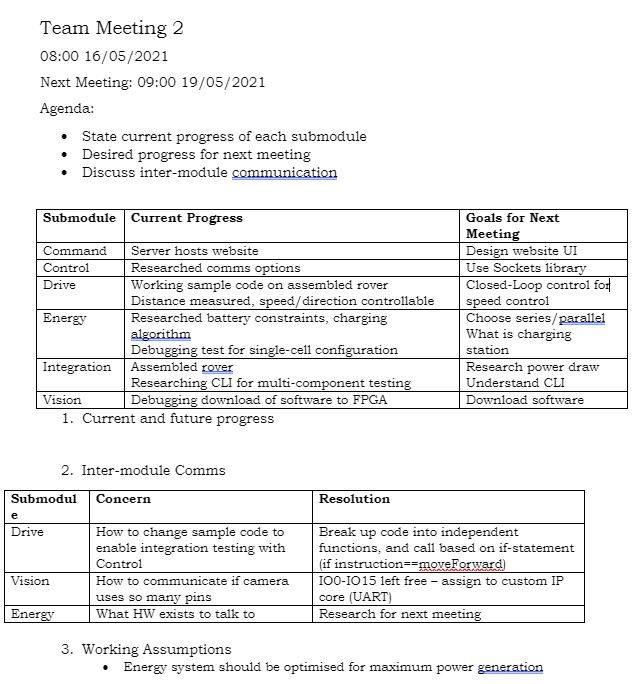
\includegraphics[scale=0.8]{Minute_sample.JPG}
\end{figure}

\subsection{Proposed wireframe website design}

\begin{figure} [h!]
    \centering
    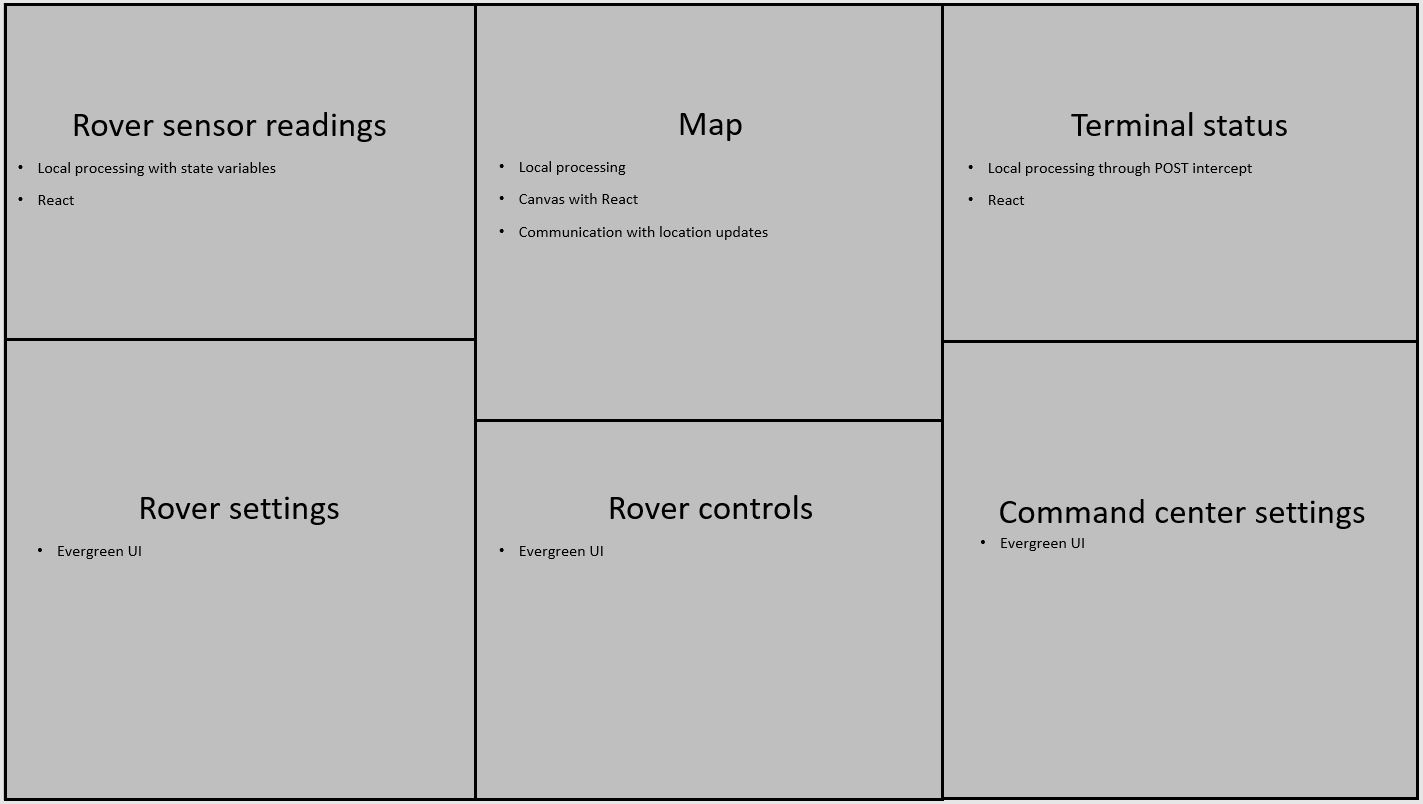
\includegraphics[scale=0.5]{Wireframe.JPG}
\end{figure}

\pagebreak
\subsection{Command module: Server code}
\begin{lstlisting}
@app.websocket("/ws/server") // Website client connection
async def websocket_client(websocket: WebSocket):
    '''
    Handle server <-> website websocket connection
    '''
    print('[Server]: Establishing command client websocket connection')
    await session_instance.client_connection.connect(websocket)
    
    try:
        while True:
            # Receive messages from command client 
            received_data = await websocket.receive_text()
                  
            if (received_data != ""):
                print("[Server Info]: Sending to rover: " + received_data)              
                await session_instance.rover_connection.send_to_rover(received_data)
            
    except WebSocketDisconnect:
        print("[Server Error]: Command client websocket terminated")


@app.websocket("/ws/rover") // Rover connection
async def websocket_endpoint(websocket: WebSocket):
    '''
    Handle server <-> rover websocket connection
    '''
    print("[Server Error]: Establishing websocket connection with rover")
    await session_instance.rover_connection.connect(websocket)
    
    try:
        while True:
            # Receive messages from the rover 
            received_data_rover = await websocket.receive_text()
            
            if (received_data_rover != ""):
                print("[Server Info]: Sending to client: " + received_data_rover)  
                await session_instance.client_connection.send_to_client(received_data_rover)
                
    except WebSocketDisconnect:
        print("[Server Error]: Rover websocket terminated")
\end{lstlisting}

\pagebreak
\subsection{Drive module: Pause feature}
\begin{lstlisting}
if(instruction[0] == 'P') { // Pause
    Stop();
    delay(100);
    Serial.write('p');
    Serial.print(String(total_x)); // Total x

    while(!Serial.available() || Serial.peek()!='N') { // Control has received 'x' value and tell 'y' to Control
    delay(1);
    }

    Serial.read(); // Remove the N
    Serial.print('y');
    Serial.print(String(total_y)); // total y

    while(!Serial.available() || Serial.peek()!='U') { // Unpause
    delay(50); // 50ms
    }
    Serial.read(); //get rid of the U
    Serial.println("Received U");
    instructionStartTime=millis();

    Serial.println("FBLRS");
    Serial.print(F); Serial.print(B); Serial.print(L); Serial.print(R); Serial.println(S);
    return;

}
\end{lstlisting}




\end{document}
